\documentclass[a4paper,12pt,oneside]{report}
\usepackage{fontspec}  
\setmainfont{Arial}      
\usepackage[vietnamese]{babel}
\usepackage{titlesec}
\usepackage{hyperref}
\usepackage{graphicx}
\usepackage{float}
\usepackage{chngcntr}
\usepackage{longtable}
\usepackage{enumitem}
\usepackage{array}
\usepackage{makecell}
\usepackage{fancyhdr}
\usepackage{tikz}
\pagestyle{empty}

\usepackage[a4paper,
    left=2.5cm,
    right=2cm,
    top=2cm,
    bottom=2cm
]{geometry}

\setcounter{secnumdepth}{3} % đánh số đến subsubsection
\setcounter{tocdepth}{3} % Table of content hiển thị đến subsubsection

\counterwithin{figure}{subsection}

\titleformat{\chapter}[hang] 
  {\normalfont\LARGE\bfseries}
  {\thechapter} 
  {1em}        
  {}             
  \renewcommand{\thechapter}{\Roman{chapter}}
\renewcommand{\thesection}{\arabic{section}}
\setlength{\parskip}{10pt} 

\begin{document}

% Vẽ khung viền
\begin{tikzpicture}[remember picture, overlay]
  \draw[line width=1pt]
    ([xshift=1cm,yshift=-1cm]current page.north west) rectangle 
    ([xshift=-1cm,yshift=1cm]current page.south east);
\end{tikzpicture}

% Nội dung chính căn giữa
\begin{center}
    \textbf{ĐẠI HỌC QUỐC GIA HÀ NỘI} \\
    \textbf{TRƯỜNG ĐẠI HỌC CÔNG NGHỆ} \\[3em]

    
\includegraphics[width=0.3\textwidth]{img/logo.png} \\[3em]

    \LARGE \textbf{BÀI TẬP LỚN} \\[0.5em]
    \Large \textbf{CÔNG NGHỆ PHẦN MỀM} \\[0.5em]
    \normalsize \textbf{Chủ đề: Hệ thống đặt phòng khách sạn} \\[4em]
\end{center}

\vspace{2em}

% Thông tin nhóm
\hfill
\begin{minipage}{0.45\textwidth}
    \textbf{Lớp:} INT2208\_7 \\
    \textbf{Nhóm:} 7 \\
    \textbf{Thành viên:}
    \begin{itemize}
        \item Phạm Đức Thiện
        \item Phạm Tuấn Việt
        \item Đoàn Văn Tuyền
        \item Phạm Văn Minh
    \end{itemize}
\end{minipage}

\vfill

\begin{center}
    \thepage
\end{center}

\tableofcontents

\chapter{Đặc tả yêu cầu}
\section{Đặt vấn đề}
Hiện nay, với sự bùng nổ của ngành du lịch, các loại hình tham quan trải nghiệm cùng sự phát triển mạnh mẽ của điện thoại thông minh, nhu cầu tìm kiếm và đặt phòng khách sạn trực tuyến tại Việt Nam cũng như trên toàn thế giới đang ngày càng gia tăng. Tuy nhiên, giữa khối lượng thông tin khổng lồ và không phải lúc nào cũng chính xác, du khách thường gặp khó khăn và mất nhiều thời gian để chọn lựa khách sạn phù hợp với nhu cầu của mình.

Chính vì vậy, chúng tôi đã phát triển ứng dụng "TravelHelper" – một công cụ đặt phòng khách sạn và phương tiện thông minh, với mục tiêu cung cấp cho du khách trong và ngoài nước một giải pháp đặt lịch tiện lợi, an toàn và tiết kiệm. Ứng dụng này cho phép người dùng tìm kiếm khách sạn và phương tiện di chuyển đáp ứng các tiêu chí như vị trí, giá cả, đánh giá, và tiện nghi, giúp du khách dễ dàng lựa chọn khách sạn phù hợp nhất với yêu cầu của mình. Bên cạnh đó, TravelHelper còn hỗ trợ chủ khách sạn trong việc cho thuê phòng, quản lý lịch đặt phòng và kết nối với khách hàng.

TravelHelper là một ứng dụng di động tương thích với cả hai nền tảng IOS và Android, tích hợp Google Maps để cung cấp bản đồ trực quan. Du khách chỉ cần kết nối Internet là có thể dễ dàng tìm kiếm thông tin về khách sạn, phương tiện di chuyển, kiểm tra giá phòng, xem đánh giá từ các khách hàng trước, và thực hiện giao dịch thanh toán trực tuyến hoặc trực tiếp một cách nhanh chóng và an toàn. Ứng dụng đảm bảo rằng lịch đặt phòng sẽ không bị hủy bỏ mà không có sự đồng ý của cả du khách và chủ khách sạn. Sau khi đặt phòng, cả du khách và chủ khách sạn đều nhận được thông báo và thông tin cần thiết để liên lạc và trao đổi thêm. Khi kết thúc kỳ nghỉ, du khách có thể để lại đánh giá về khách sạn và các đánh giá này sẽ được công khai để giúp các du khách khác dễ dàng tham khảo. Chủ khách sạn cần xác thực thông tin để đăng ký sử dụng dịch vụ cho thuê khách sạn, vì vậy có thể đảm bảo được sự an toàn và minh bạch cho du khách.

Đối tượng người dùng của TravelHelper là bất kỳ ai có nhu cầu đặt phòng khách sạn qua điện thoại thông minh, từ du khách trong nước đến quốc tế. Ứng dụng hỗ trợ nhiều ngôn ngữ, bao gồm Tiếng Việt và Tiếng Anh, và sẽ mở rộng thêm các ngôn ngữ khác trong tương lai.

\section{Bảng thuật ngữ}
Bảng thuật ngữ xác định các thuật ngữ cụ thể cho ứng dụng TravelHelper, giải thích các thuật ngữ người đọc có thể không biết trong mô tả ca sử dụng và các tài liệu khác.

\textbf{Người dùng:}\\
\indent
Là người sử dụng hệ thống, có thể có hoặc không có tài khoản của hệ thống. Bao gồm cả du khách và chủ khách sạn.

\textbf{Hệ quản trị cơ sở dữ liệu:}\\
\indent
Là phần mềm quản lý, tổ chức và điều phối các hoạt động liên quan đến cơ sở dữ liệu, bao gồm lưu trữ, truy vấn, cập nhật và bảo mật dữ liệu.

\textbf{Cơ sở dữ liệu:}\\
\indent Là một tập hợp dữ liệu được tổ chức, lưu trữ và quản lý một cách có cấu trúc, cho phép dễ dàng truy xuất, cập nhật và xử lý thông tin.

\textbf{API Bản đồ (Google Map API): }\\
\indent Là API bản đồ được tích hợp cho hệ thống, có chức năng định vị và xác định các vị trí của khách sạn, phòng, địa điểm du lịch và hướng dẫn đường đi cho người dùng.

\textbf{Hệ thống thanh toán:}\\
\indent Là hệ thống con có thể truy cập, truy vấn và xử lý cơ sở dữ liệu thanh toán và hóa đơn. Hệ thống này hỗ trợ các phương thức thanh toán như thẻ tín dụng, thẻ ghi nợ, ví điện tử và thanh toán trực tuyến.

\textbf{Khách sạn: }\\
\indent Là cơ sở lưu trú phục vụ cho du khách với các dịch vụ phòng ngủ, nhà hàng, giải trí và các tiện ích khác.
Phòng: Là một đơn vị cung cấp chỗ ở trong khách sạn, có thể được phân theo loại phòng (phòng đơn, phòng đôi, phòng suite) và mức giá.

\textbf{Phương tiện: }\\
\indent Là các dịch vụ di chuyển được hệ thống cung cấp như máy bay, taxi, xe bus,...
Du khách: Là người dùng hệ thống với mục đích đặt phòng và phương tiện.

\textbf{Chủ khách sạn: }\\
\indent Là người dùng hệ thống với mục đích cho thuê phòng khách sạn.

\textbf{Đánh giá khách sạn: }\\
\indent Là quá trình mà du khách cung cấp ý kiến về trải nghiệm của mình tại khách sạn, bao gồm các yếu tố như chất lượng phòng. Các đánh giá có thể được hiển thị công khai để hỗ trợ các khách hàng khác trong việc lựa chọn khách sạn.

\textbf{Đặt phòng: }\\
\indent Là hành động mà người dùng lựa chọn và xác nhận việc thuê phòng tại một khách sạn vào một thời điểm nhất định thông qua hệ thống.

\textbf{Cho thuê phòng: }\\
\indent Chủ khách sạn cung cấp dịch vụ đặt phòng trên hệ thống.
Đặt phương tiện: Là hành động của du khách lựa chọn đặt vé trước của một phương tiện.

\textbf{Hủy phòng: }\\
\indent Là hành động người dùng yêu cầu hủy bỏ đơn đặt phòng đã xác nhận. Các quy định về hủy phòng có thể áp dụng phí hủy dựa trên thời gian yêu cầu hủy.

\textbf{Tìm kiếm phòng: }\\
\indent Là tính năng cho phép người dùng tìm kiếm các phòng khách sạn có sẵn dựa trên các tiêu chí như địa điểm, loại phòng, giá cả và thời gian lưu trú.

\section{Đặc tả bổ sung}
\textbf{\indent Mục tiêu}\\
\indent Mục đích của tài liệu này là xác định các yêu cầu của ứng dụng đặt phòng khách sạn TravelHelper. Đặc tả bổ sung này liệt kê các yêu cầu nằm ngoài mô hình usecase để hoàn thiện các chức năng cần đạt được của hệ thống.

\textbf{Phạm vi}\\
\indent Đặc tả bổ sung này áp dụng cho ứng dụng TravelHelper. Đặc tả này xác định các yêu cầu phi chức năng của ứng dụng; chẳng hạn như độ tin cậy, khả năng sử dụng, hiệu suất và khả năng hỗ trợ, cũng như các yêu cầu chức năng chung trong một số Use Case.

\textbf{Chức năng}\\
\indent Nhiều người dùng có thể dùng ứng dụng cùng lúc. 

\textbf{Tính khả dụng}\\
\indent Hệ thống sẽ dễ dàng tương tác, các tác vụ xử lý nhanh, hoạt động trên cả hệ điều hành Android và IOS. Hệ thống yêu cầu kết nối mạng để truy cập.

\textbf{Tính tin cậy}\\
\indent Hệ thống có thể sử dụng 24/7, đáp ứng được tần suất truy cập cao.

\textbf{Tính bảo mật}\\
\indent Hệ thống ngăn chặn các hành vi truy cập và đánh cắp dữ liệu trái phép. Hệ thống đảm bảo chỉ chủ tài khoản mới có thể nhìn thấy thông tin cá nhân của bản thân. Chỉ có chủ mới có thể thay đổi thông tin phòng.

\textbf{Ràng buộc thiết kế}\\
\indent Hệ thống cung cấp giao diện cho điện thoại thông minh.
\section{Mô hình Use Case}
\subsection{Danh sách tác nhân}

\begin{figure}[H]
    \centering
    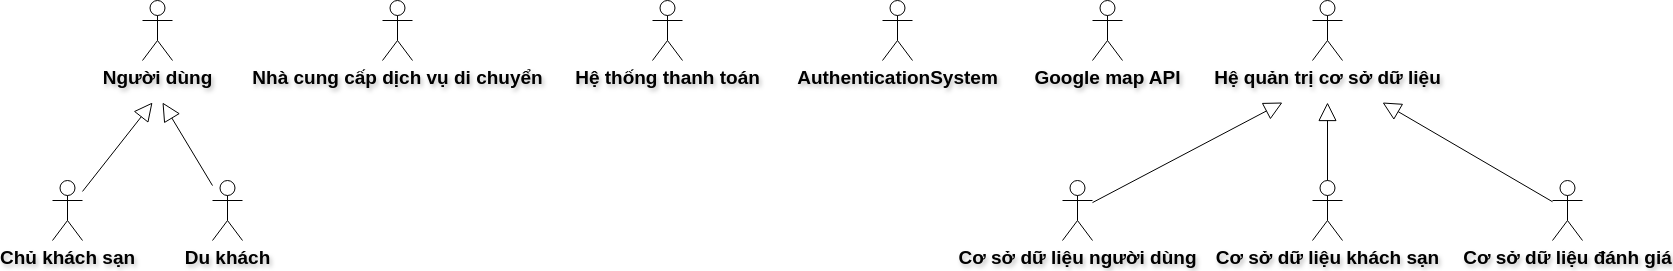
\includegraphics[width=\textwidth]{img/Use_Case-Actor.drawio.png} 
    \caption{ Biểu đồ ca sử dụng về tác nhân và sự phụ thuộc lẫn nhau giữa các tác nhân}
    \label{fig:actors}
\end{figure}

Danh sách các tác nhân của hệ thống bao gồm: 
\begin{itemize}
    \item \textbf{Người dùng:} là khách hàng sử dụng ứng dụng gồm 2 loại là du khách(người dùng với mục đích đặt phòng và phương tiện) và chủ khách sạn(người dùng với mục đích cho thuê và quản lý phòng khách sạn)
    \item \textbf{Nhà cung cấp dịch vụ di chuyển:} là các công ty vận chuyển như taxi, xe buýt, máy bay. Được tích hợp với hệ thống để hiển thị các lựa chọn phương tiện di chuyển và thực hiện thanh toán.
    \item \textbf{Hệ thống thanh toán:} xử lý giao dịch tài chính giữa người dùng với chủ khách sạn hoặc nhà cung cấp dịch vụ vận chuyển.
    \item \textbf{Hệ quản trị cơ sở dữ liệu:} là phần mềm cung cấp dịch vụ quản lý cơ sở dữ liệu. Trong đó có 3 cơ sở dữ liệu chính: cơ sở dữ liệu người dùng, cơ sở dữ liệu khách sạn, cơ sở dữ liệu đánh giá.
    \item \textbf{AuthenticationSystem:} là phần mềm cung cấp dịch vụ xác thực người dùng và khách sạn như CCCD, giấy xác nhận kinh doanh.
    \item \textbf{Google map API:} API cung cấp khả năng tích hợp bản đồ và định vị vào ứng dụng.
\end{itemize}

\subsection{Các ca sử dụng bậc cao}
\begin{figure}[H]
    \centering
    \includegraphics[width=\textwidth]{img/Use_Case-Usecase bậc cao.drawio.png} 
    \caption{Biểu đồ ca sử dụng bậc cao}
\end{figure}
Tác nhân người dùng sử dụng ứng dụng để đặt lịch trực tuyến. Các ca sử dụng bậc cao bao gồm \textbf{Tra cứu phòng, Tra cứu phương tiện, Cho thuê phòng, Theo dõi phòng đã thuê, Theo dõi phương tiện đã thuê, Theo dõi phòng đang cho thuê} và \textbf{Thanh toán}. Tra cứu phòng và tra cứu phương tiện dành cho du khách muốn tìm kiếm và thuê các loại hình dịch vụ này. Theo dõi phòng và theo dõi phương tiện đã thuê dành cho du khách đã thực hiện thuê và muốn kiểm tra tình trạng các dịch vụ. Cho thuê phòng và theo dõi phòng đang cho thuê dành cho chủ khách sạn muốn cung cấp dịch vụ khách sạn và quản lý dịch vụ của mình. Thanh toán là ca sử dụng phát sinh khi người dùng đã thuê một dịch vụ mất phí như phòng khách sạn và phương tiện và dùng để thanh toán cho các dịch vụ này.

\subsection{Các ca sử dụng dưới góc nhìn người dùng}
\begin{figure}[H]
    \centering
    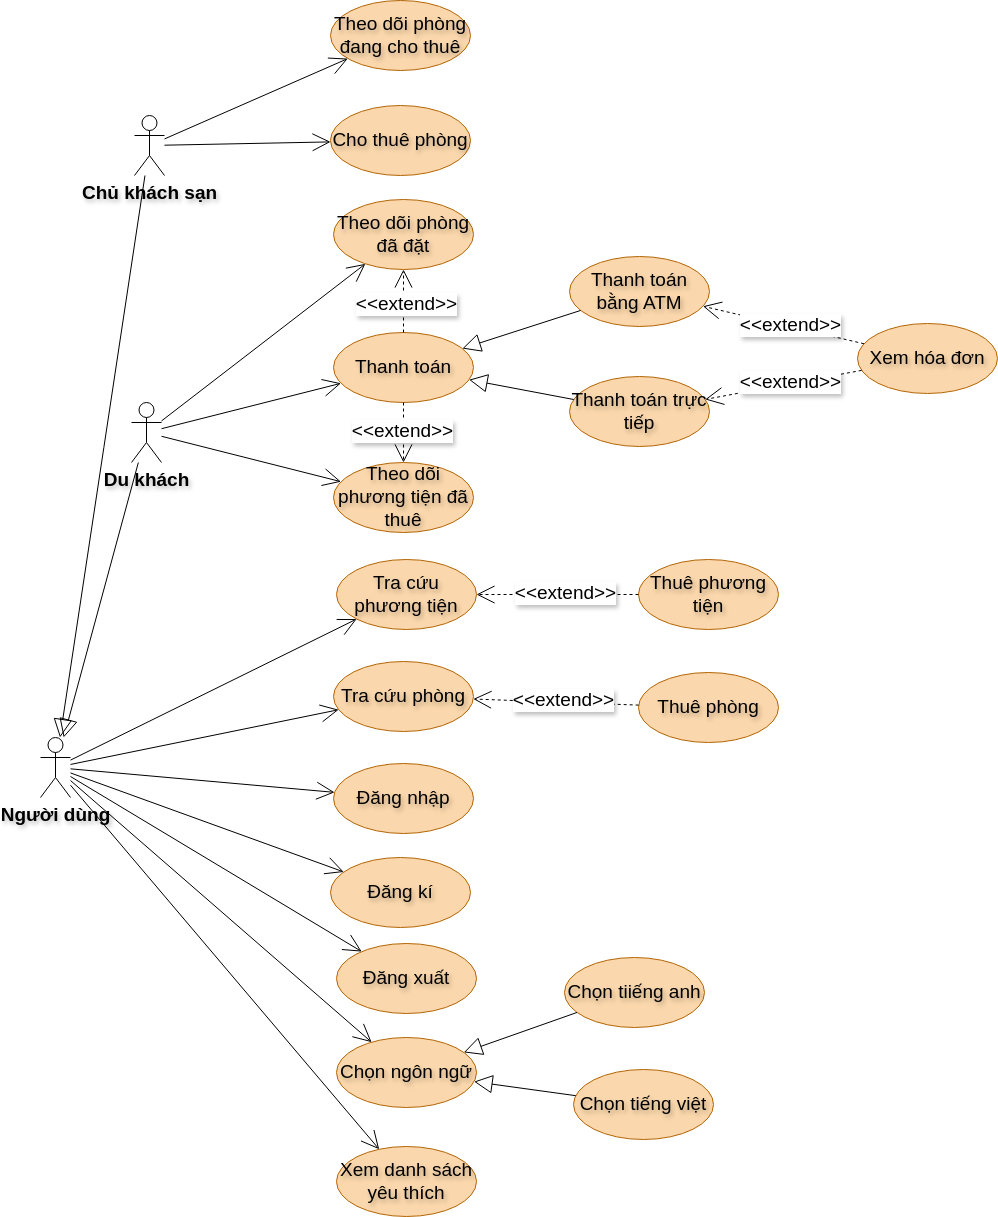
\includegraphics[width=0.95\textwidth]{img/Use_Case-Use case dưới góc nhìn người sử dụng.drawio.png} 
    \caption{Biểu đồ ca sử dụng dưới góc nhìn của Người dùng}
\end{figure}
Ca sử dụng dưới góc nhìn người dùng phân tích cụ thể các hoạt động và mục tiêu của người dùng khi sử dụng các ca sử dụng và bổ sung thêm các chi tiết cho biểu đồ ca sử dụng bậc cao. 
\subsection{Ca sử dụng Đăng nhập}
\begin{figure}[H]
    \centering
    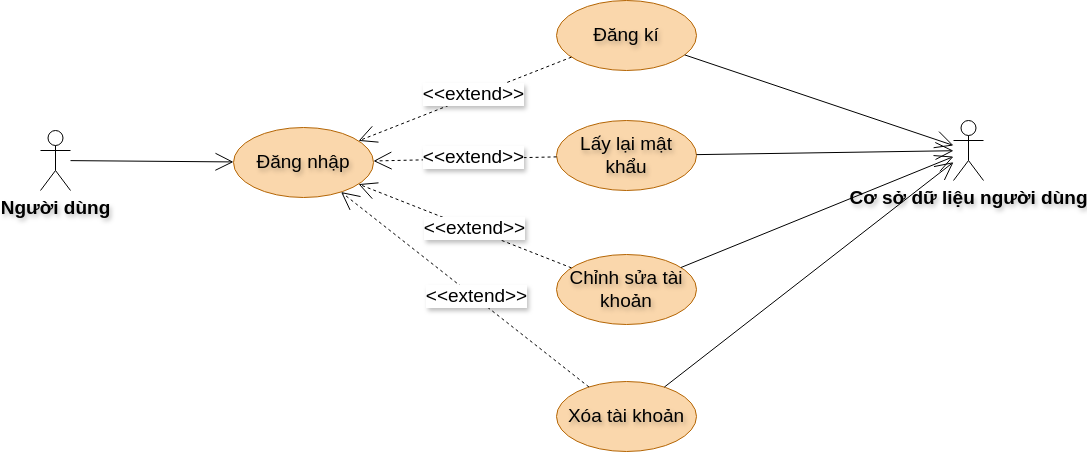
\includegraphics[width=\textwidth]{img/Use_Case-Đăng nhập.drawio.png}
    \caption{Biểu đồ ca sử dụng Đăng nhập}
\end{figure}
Ca sử dụng \textbf{Đăng nhập} có thể dùng sau khi người dùng đã đăng ký, người dùng có thể lựa chọn các tùy chọn thêm như lấy lại mật khẩu và ghi nhớ mật khẩu ở ca sử dụng này.

\subsection{Ca sử dụng Tra cứu thông tin phòng khách sạn}
\begin{figure}[H]
    \centering
    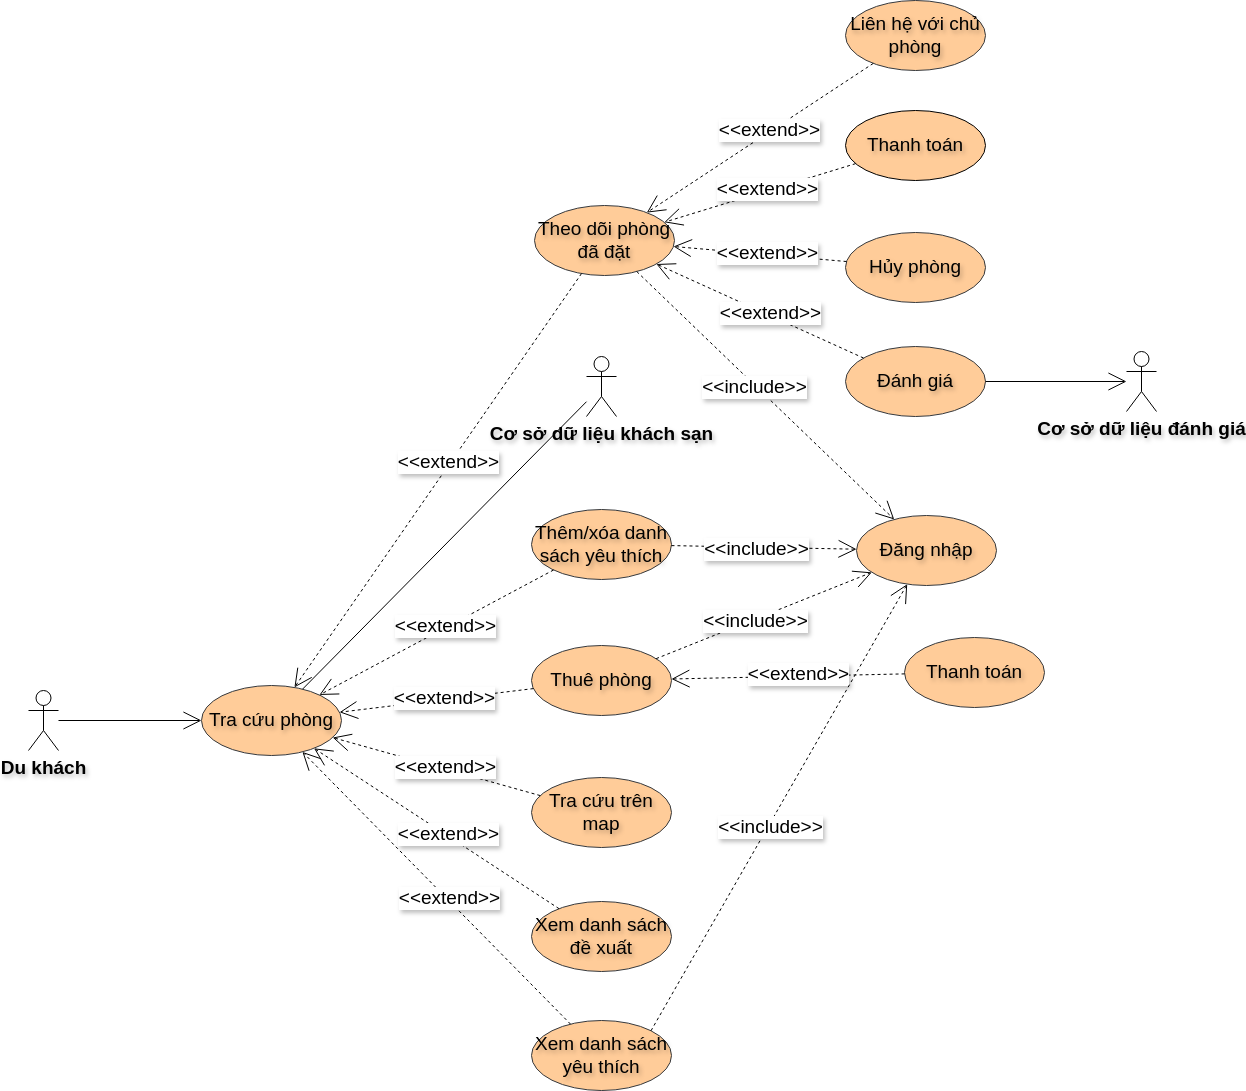
\includegraphics[width=\textwidth]{img/Use_Case-Tra cứu phòng.drawio.png}
    \caption{Biểu đồ ca sử dụng Tra cứu thông tin phòng khách sạn
}
\end{figure}
Ca sử dụng \textbf{Tra cứu phòng} được người dùng sử dụng khi muốn tìm kiếm thông tin về phòng khách sạn. Người dùng cần phải đăng nhập để có thể sử dụng các tính năng bổ sung như cập nhật và xem danh sách yêu thích, đặt phòng và theo dõi phòng đã đặt. Người dùng cũng được cung cấp dịch vụ tìm phòng trên bản đồ trực quan thông qua dịch vụ của Google map.

\subsection{Ca sử dụng Tra cứu thông tin phương tiện di chuyển}
\begin{figure}[H]
    \centering
    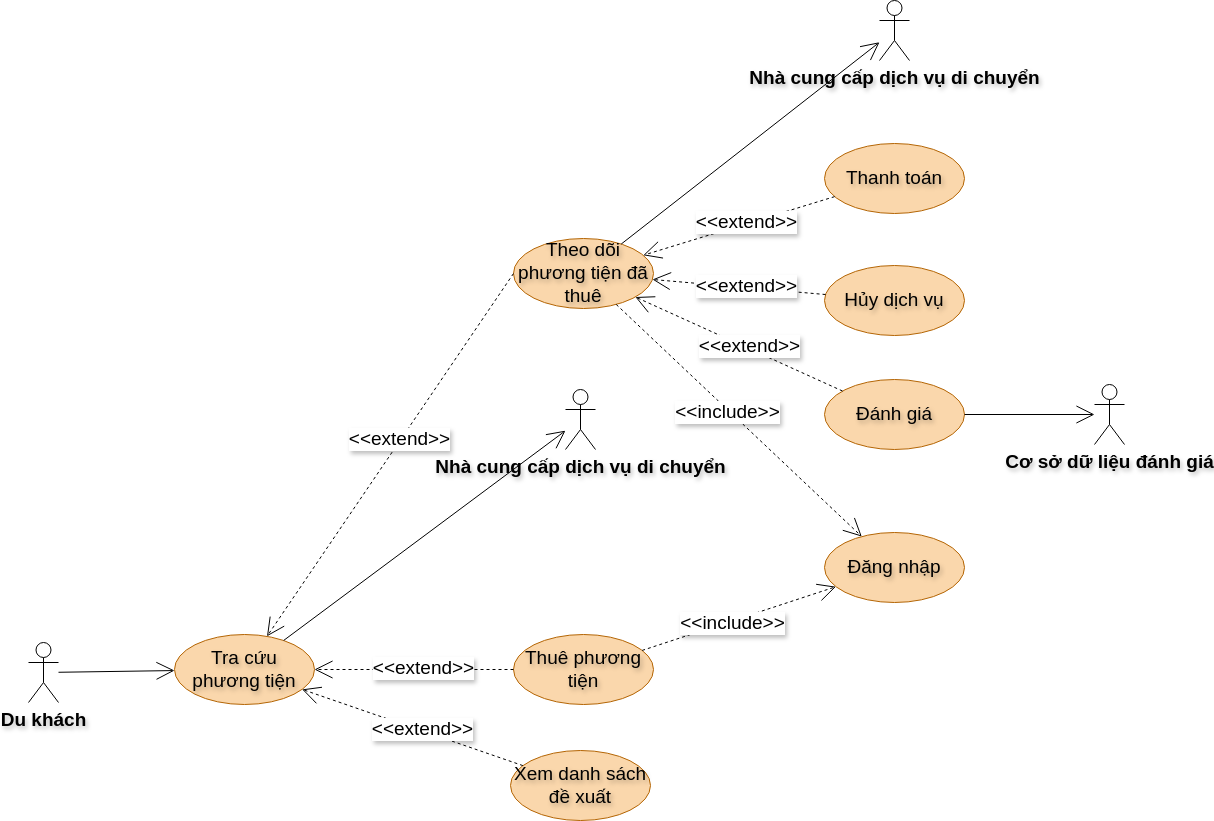
\includegraphics[width=0.9\textwidth]{img/Use_Case-Tra cứu phương tiện.drawio.png}
    \caption{Biểu đồ ca sử dụng Tra cứu thông tin phương tiện}
\end{figure}
Ca sử dụng \textbf{Tra cứu phương tiện} được người dùng sử dụng khi muốn tìm kiếm thông tin về phương tiện di chuyển. Người dùng cần phải đăng nhập để có thể sử dụng các tính năng bổ sung như đặt phương tiện và theo dõi phương tiện đã đặt.

\subsection{Ca sử dụng Cho thuê phòng}
\begin{figure}[H]
    \centering
    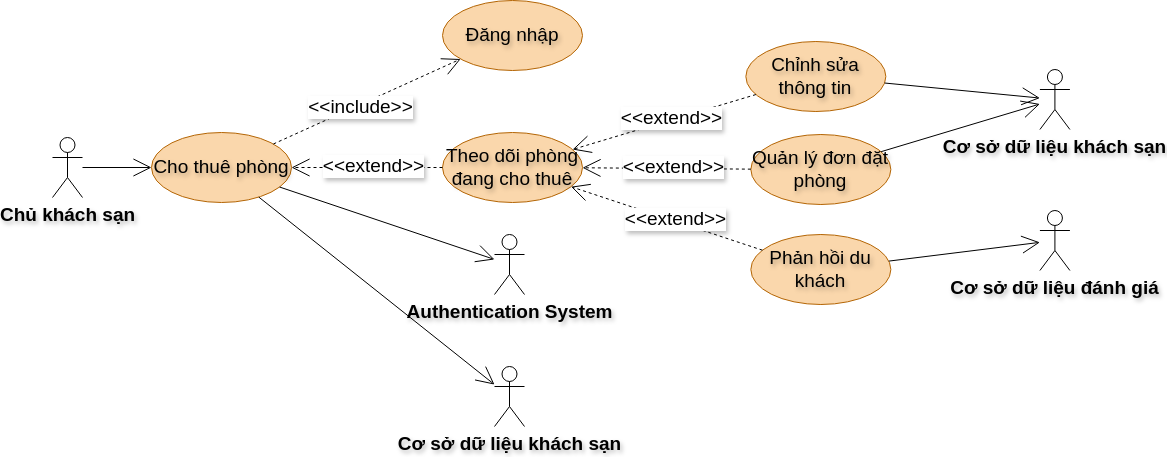
\includegraphics[width=0.8\textwidth]{img/Use_Case-Cho thuê phòng.drawio.png}
    \caption{Biểu đồ ca sử dụng Cho thuê phòng}
\end{figure}
Ca sử dụng \textbf{Cho thuê phòng} được người dùng chủ khách sạn đã xác thực tài khoản sử dụng để cung cấp dịch vụ phòng khách sạn cho du khách và quản lý khách sạn đang cho thuê.

\section{Đặc tả Use Case}
\subsection{Đặt phòng khách sạn}
\begin{figure}[H]
    \centering
    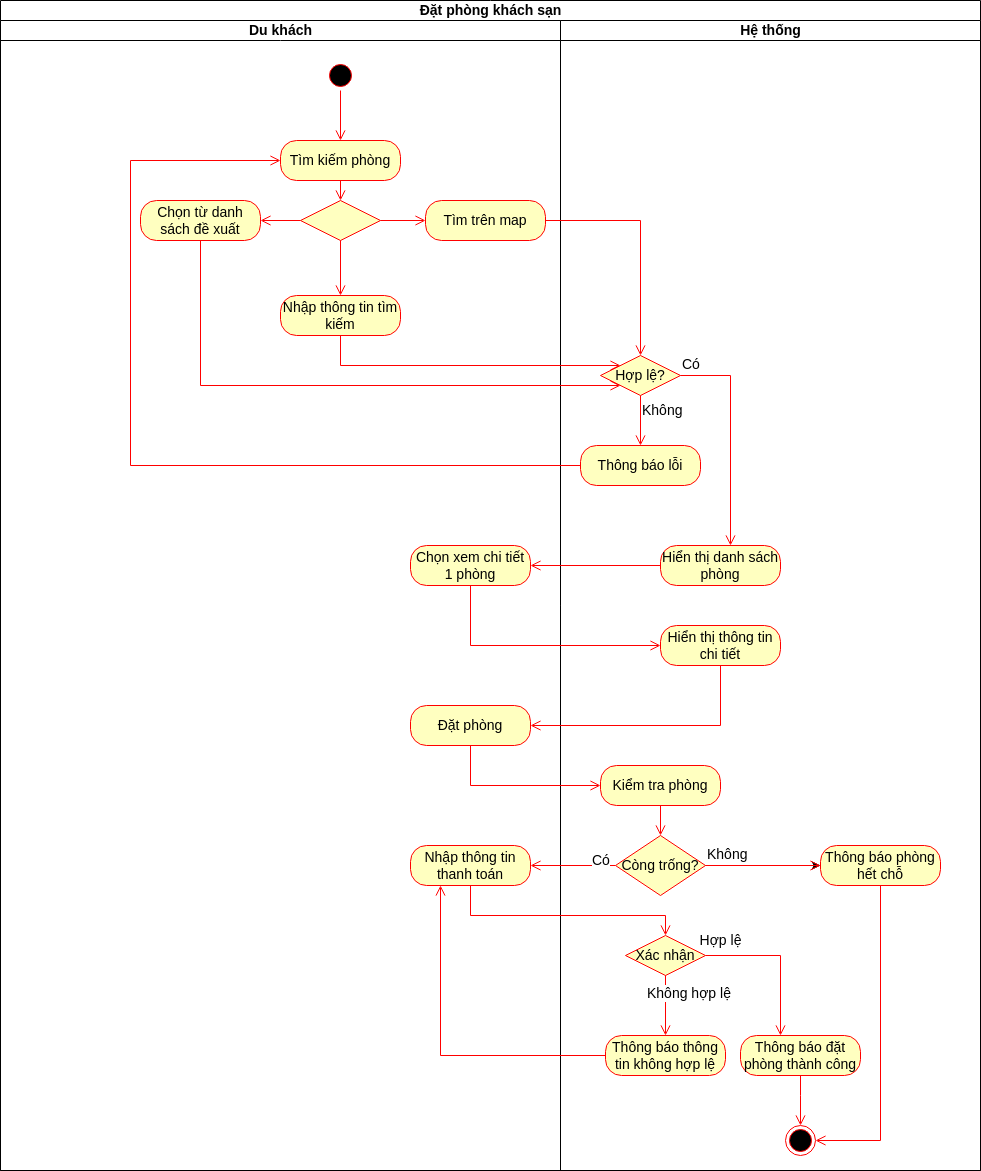
\includegraphics[width=\textwidth]{img/1.Tuyền-Đặt phòng.drawio.png}
    \caption{Biểu đồ hoạt động ca sử dụng Đặt phòng khách sạn}
\end{figure}
\textbf{\indent Mô tả}\\
\indent Chức năng này cho phép người dùng tìm kiếm phòng dựa trên các tiêu chí như vị trí, giá cả, tiện nghi, đánh giá... Người dùng có thể xem chi tiết phòng và tiến hành đặt phòng.


\textbf{Các tác nhân}
\begin{itemize}
    \item \textbf{Du khách:} Tìm kiếm và đặt phòng.
    \item \textbf{Cơ sở dữ liệu khách sạn:} Lưu trữ và cung cấp dữ liệu về các phòng khách sạn.
\end{itemize}

\textbf{Điều kiện kích hoạt ca sử dụng}
\begin{itemize}
    \item Người dùng đã đăng nhập vào hệ thống.
\end{itemize}

\textbf{Tiền điều kiện}
\begin{itemize}
    \item Hệ thống đã có dữ liệu phòng.
    \item Kết nối mạng ổn định.
\end{itemize}

\textbf{Hậu điều kiện}
\begin{itemize}
    \item Nếu đặt phòng thành công, thông tin đặt phòng được lưu lại.
    \item Nếu chỉ tìm kiếm, hệ thống có thể lưu lại lịch sử tìm kiếm để gợi ý sau này.
\end{itemize}

\textbf{Các luồng sự kiện}

\begin{small}
\textbf{Luồng cơ bản}\\
\indent 1. Người dùng chọn tìm kiếm phòng theo các phương thức như theo thông tin, tìm kiếm trên map, chọn từ danh sách đề xuất.\\
\indent 2. Hệ thống kiểm tra tính hợp lệ của thông tin khách sạn.\\
\indent 3. Hệ thống hiển thị danh sách phòng theo yêu cầu của du khách.\\
\indent 4. Du khách chọn một phòng để xem chi tiết.\\
\indent 5. Hệ thống hiển thị thông tin chi tiết của phòng đã chọn.\\
\indent 6. Người dùng chọn đặt phòng.\\
\indent 7. Hệ thống kiểm tra xem phòng còn trống không.\\
\indent 8. Người dùng nhập thông tin tài khoản và xác nhận đặt phòng.\\
\indent 9. Hệ thống xác nhận thông tin thanh toán.\\
\indent 10. Hệ thống hiển thị thông báo thành công và kết thúc ca sử dụng.\\

\textbf{Luồng thay thế}\\
\indent 2.1 Nếu thông tin không hợp lệ, hệ thống thông báo và quay lại bước 1.\\
\indent 7.1 Nếu phòng đã hết chỗ thì hệ thống hiện thông báo và kết thúc ca sử dụng.\\
\indent 9.1 Nếu thông tin thanh toán không hợp lệ, hệ thống hiển thị thông báo và quay lại bước 8.\\
\end{small}\\
\textbf{\indent Business rules}
\begin{itemize}
    \item Chỉ hiển thị phòng khả dụng trong khoảng thời gian người dùng yêu cầu.
    \item Nếu người dùng hủy đặt phòng, áp dụng chính sách hoàn tiền của từng phòng.
    \item Có thể có giá ưu đãi cho khách hàng thân thiết hoặc đặt phòng sớm.
\end{itemize}

\textbf{Yêu cầu phi chức năng}
\begin{itemize}
    \item Tốc độ tìm kiếm nhanh, tối ưu thời gian phản hồi dưới 3 giây.
    \item Giao diện thân thiện, hiển thị rõ ràng thông tin quan trọng.
\end{itemize}

\textbf{Extension point}
\begin{itemize}
    \item Hệ thống có thể tích hợp AI để đề xuất phòng phù hợp dựa trên lịch sử tìm kiếm.
    \item Hỗ trợ bản đồ tương tác để tìm kiếm phòng theo vị trí trực quan.
\end{itemize}

\subsection{Theo dõi phòng đã đặt}
\begin{figure}[H]
    \centering
    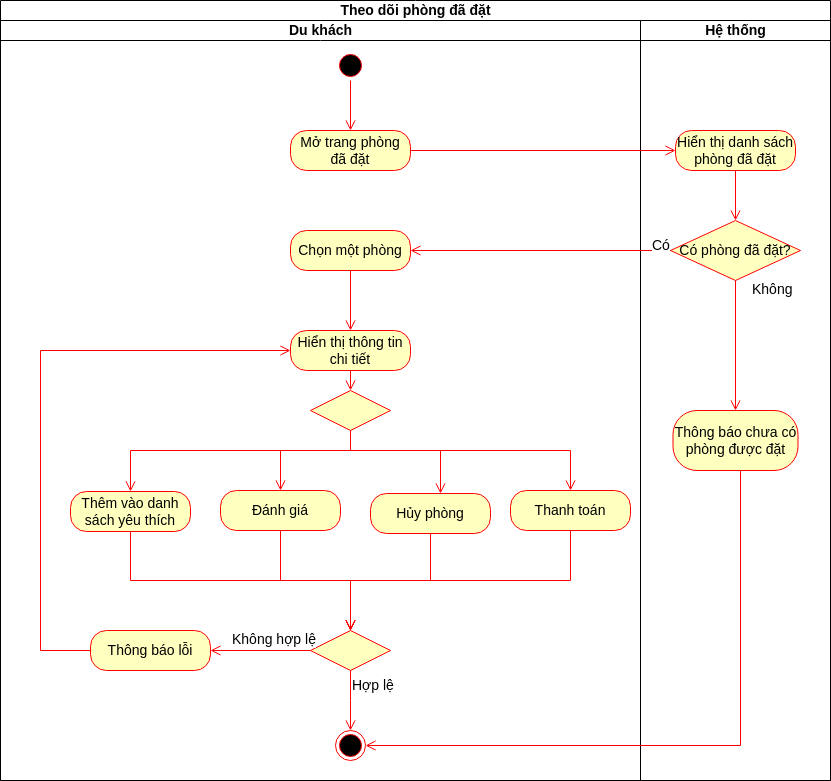
\includegraphics[width=0.95\textwidth]{img/1.Tuyền-Tra cứu thông tin phòng đã thuê.drawio.png}
    \caption{Biểu đồ hoạt động ca sử dụng Theo dõi phòng đã đặt}
\end{figure}
\textbf{\indent Mô tả}\\
\indent Chức năng này cho phép người dùng xem danh sách phòng đã thuê, kiểm tra thông tin đặt phòng và hủy đặt phòng nếu cần.

\textbf{Các tác nhân}
\begin{itemize}
    \item \textbf{Du khách:}  Xem danh sách và chi tiết phòng đã thuê.
\end{itemize}

\textbf{Điều kiện kích hoạt ca sử dụng}
\begin{itemize}
    \item Người dùng đã đăng nhập vào hệ thống.
\end{itemize}

\textbf{Tiền điều kiện}
\begin{itemize}
    \item Người dùng đã có ít nhất một phòng được đặt trước đó.
\end{itemize}

\textbf{Hậu điều kiện}
\begin{itemize}
    \item Nếu người dùng chỉ xem, không có thay đổi nào trong dữ liệu đặt phòng.
    \item Nếu người dùng hủy phòng, hệ thống cập nhật trạng thái đặt phòng và hoàn tiền (nếu chính sách cho phép).
\end{itemize}

\textbf{Các luồng sự kiện}

\begin{small}
\textbf{Luồng cơ bản}\\
\indent 1. Người dùng mở trang “Phòng đã đặt”.\\
\indent 2. Hệ thống hiển thị danh sách các phòng đã đặt.\\
\indent 3. Người dùng chọn một phòng để xem chi tiết.\\
\indent 4. Hệ thống hiển thị thông tin đặt phòng.\\
\indent 5. Người dùng có thể thao tác hủy phòng, thanh toán, đánh giá và thêm vào danh sách yêu thích.\\
\indent 6. Hệ thống xử lý yêu cầu và hiển thị kết quả.\\

\textbf{Luồng thay thế}\\
\indent 2.1 Nếu người dùng chưa đặt phòng nào, hệ thống hiển thị thông báo “Bạn chưa có phòng nào được đặt”.\\
\indent 6.1 Nếu yêu cầu không hợp lệ hoặc không phù hợp với chính sách thì thông báo lỗi và quay lại bước 4.\\
\end{small}\\
\textbf{\indent Business rules}
\begin{itemize}
    \item Chỉ cho phép hủy phòng trước thời gian check-in theo chính sách của từng phòng.
    \item Hiển thị đầy đủ thông tin về lịch sử đặt phòng, bao gồm cả những phòng đã hoàn thành.
\end{itemize}

\textbf{Yêu cầu phi chức năng}
\begin{itemize}
    \item Giao diện hiển thị rõ ràng, dễ dàng điều hướng giữa các phòng đã đặt.
\end{itemize}

\textbf{Extension point}
\begin{itemize}
    \item Hệ thống có thể hiển thị lịch trình check-in/check-out sắp tới.
    \item Hỗ trợ xuất hóa đơn điện tử cho khách hàng.
\end{itemize}


\subsection{Đánh giá phòng đã thuê}
\begin{figure}[H]
    \centering
    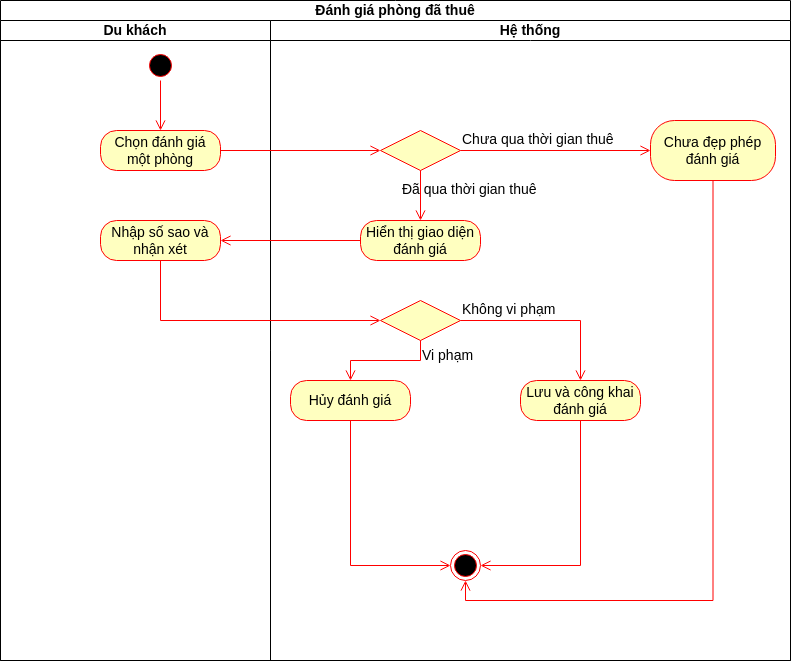
\includegraphics[width=\textwidth]{img/1.Tuyền-Đánh giá phòng đã thuê.drawio.png}
    \caption{Biểu đồ hoạt động cho ca sử dụng Đánh giá phòng đã thuê}
\end{figure}
\textbf{\indent Mô tả}\\
\indent Sau khi thuê phòng, người dùng có thể đánh giá bằng số sao và viết nhận xét về trải nghiệm của mình.

\textbf{Các tác nhân}
\begin{itemize}
    \item \textbf{Người dùng:} Đánh giá phòng đã thuê.
\end{itemize}

\textbf{Điều kiện kích hoạt ca sử dụng}
\begin{itemize}
    \item Người dùng đã hoàn thành ít nhất một lần thuê phòng.
\end{itemize}

\textbf{Tiền điều kiện}
\begin{itemize}
    \item Phòng đã qua thời gian thuê (không cho phép đánh giá trước khi trải nghiệm).
\end{itemize}

\textbf{Hậu điều kiện}
\begin{itemize}
    \item Đánh giá được lưu và hiển thị trên trang phòng.
\end{itemize}

\textbf{Các luồng sự kiện}

\begin{small}
\textbf{Luồng cơ bản}\\
\indent 1. Người dùng chọn đánh giá phòng đã thuê.\\
\indent 2. Hệ thống kiểm tra phòng có đủ điều kiện để đánh giá chưa.\\
\indent 3. Người dùng nhập số sao và nhận xét.\\
\indent 4. Hệ thống kiểm tra đánh giá.\\
\indent 5. Hệ thống lưu đánh giá và hiển thị công khai.\\

\textbf{Luồng thay thế}\\
\indent 2.1 Nếu phòng chưa qua thời gian thuê, hệ thống không cho phép đánh giá.\\
\indent 4.1 Nếu đánh giá chứa nội dung vi phạm, hệ thống từ chối lưu.\\
\end{small}\\
\textbf{\indent Business rules}
\begin{itemize}
    \item Mỗi phòng chỉ có thể được đánh giá sau khi thời gian thuê kết thúc.
    \item Không cho phép chỉnh sửa hoặc xóa đánh giá sau khi đã gửi.
\end{itemize}

\textbf{Yêu cầu phi chức năng}
\begin{itemize}
    \item Đánh giá hiển thị theo thời gian thực, phản hồi nhanh.
\end{itemize}

\textbf{Extension point}
\begin{itemize}
    \item Hệ thống có thể đề xuất các phòng tương tự dựa trên đánh giá của người dùng.
\end{itemize}



\subsection{Liên hệ với chủ khách sạn}
\begin{figure}[H]
    \centering
    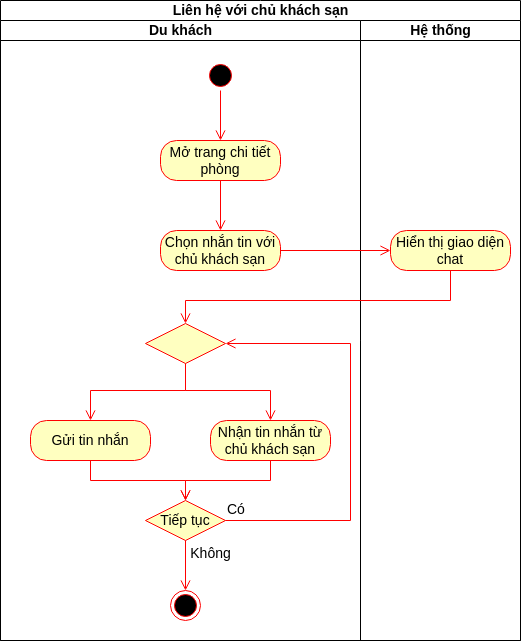
\includegraphics[width=0.7\textwidth]{img/1.Tuyền-Chat với chủ phòng.drawio.png}
    \caption{Biểu đồ hoạt động cho ca sử dụng Liên hệ với chủ khách sạn}
\end{figure}
\textbf{\indent Mô tả}\\
\indent Người dùng có thể chat trực tiếp với chủ phòng để đặt câu hỏi về phòng hoặc yêu cầu hỗ trợ trong quá trình thuê.

\textbf{Các tác nhân}
\begin{itemize}
    \item \textbf{Người dùng (Khách hàng):} Gửi tin nhắn.
    \item \textbf{Chủ khách sạn:} Trả lời tin nhắn.
\end{itemize}

\textbf{Điều kiện kích hoạt ca sử dụng}
\begin{itemize}
    \item Người dùng đã đăng nhập.
    \item Người dùng đang xem một phòng cụ thể hoặc đã thuê phòng đó.
\end{itemize}

\textbf{Tiền điều kiện}
\begin{itemize}
    \item Chủ phòng có bật tính năng nhắn tin.
\end{itemize}

\textbf{Hậu điều kiện}
\begin{itemize}
    \item Tin nhắn được lưu lại để người dùng có thể xem lại sau.
\end{itemize}

\textbf{Các luồng sự kiện}

\begin{small}
\textbf{Luồng cơ bản}\\
\indent 1. Người dùng mở trang chi tiết phòng.\\
\indent 2. Người dùng nhấn vào nút "Nhắn tin với chủ phòng".\\
\indent 3. Hệ thống mở giao diện chat.\\
\indent 4. Người dùng gửi và nhận tin nhắn với chủ khách sạn.\\
\indent 5. Người dùng chọn kết thúc trò chuyện.\\
\end{small}\\
\textbf{\indent Business rules}
\begin{itemize}
    \item Hệ thống chỉ cho phép nhắn tin giữa khách hàng và chủ phòng khi có liên quan đến một phòng cụ thể.
    \item Không cho phép gửi nội dung vi phạm chính sách nền tảng.
\end{itemize}

\textbf{Yêu cầu phi chức năng}
\begin{itemize}
    \item Tin nhắn phải hiển thị ngay lập tức (real-time).
\end{itemize}

\textbf{Extension point}
\begin{itemize}
    \item Hệ thống có thể tích hợp chatbot AI để hỗ trợ tự động trả lời các câu hỏi phổ biến.
\end{itemize}



\subsection{Xem danh sách phòng yêu thích}
\begin{figure}[H]
    \centering
    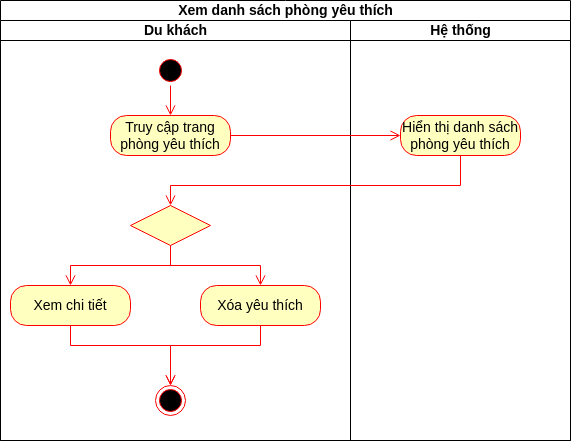
\includegraphics[width=\textwidth]{img/1.Tuyền-Xem danh sách phòng yêu thích.drawio.png}
    \caption{Biểu đồ hoạt động cho ca sử dụng Xem danh sách phòng yêu thích}
\end{figure}
\textbf{\indent Mô tả}\\
\indent Chức năng này cho phép người dùng lưu các phòng yêu thích để xem lại sau mà không cần tìm kiếm lại. Đồng thời, người dùng có thể truy cập danh sách này để quản lý các phòng đã lưu.

\textbf{Các tác nhân}
\begin{itemize}
    \item \textbf{Người dùng (Khách hàng):} Lưu, xem và xóa phòng yêu thích.
\end{itemize}

\textbf{Điều kiện kích hoạt ca sử dụng}
\begin{itemize}
    \item Người dùng đã đăng nhập vào hệ thống.
\end{itemize}

\textbf{Tiền điều kiện}
\begin{itemize}
    \item Hệ thống có dữ liệu phòng hợp lệ.
\end{itemize}

\textbf{Hậu điều kiện}
\begin{itemize}
    \item Nếu người dùng lưu phòng, phòng được thêm vào danh sách yêu thích.
    \item Nếu người dùng xóa phòng khỏi danh sách, hệ thống cập nhật lại danh sách.
\end{itemize}

\textbf{Các luồng sự kiện}

\begin{small}
\textbf{Luồng cơ bản}\\
\indent 1. Người dùng truy cập trang phòng yêu thích\\
\indent 2. Hiển thị danh sách phòng yêu thích\\
\indent 3. Người dùng có thể xem chi tiết phòng hoặc xóa phòng khỏi danh sách yêu thích.\\
\end{small}\\
\textbf{\indent Business rules}
\begin{itemize}
    \item Người dùng có thể lưu nhiều phòng mà không bị giới hạn.
    \item Nếu một phòng bị chủ phòng xóa khỏi hệ thống, nó cũng bị xóa khỏi danh sách yêu thích của người dùng.
\end{itemize}

\textbf{Yêu cầu phi chức năng}
\begin{itemize}
    \item Danh sách yêu thích phải tải nhanh, không làm gián đoạn trải nghiệm người dùng.
\end{itemize}

\textbf{Extension point}
\begin{itemize}
    \item Hệ thống có thể gợi ý các phòng tương tự dựa trên danh sách yêu thích của người dùng.
\end{itemize}



\subsection{Cho thuê phòng}
\begin{figure}[H]
    \centering
    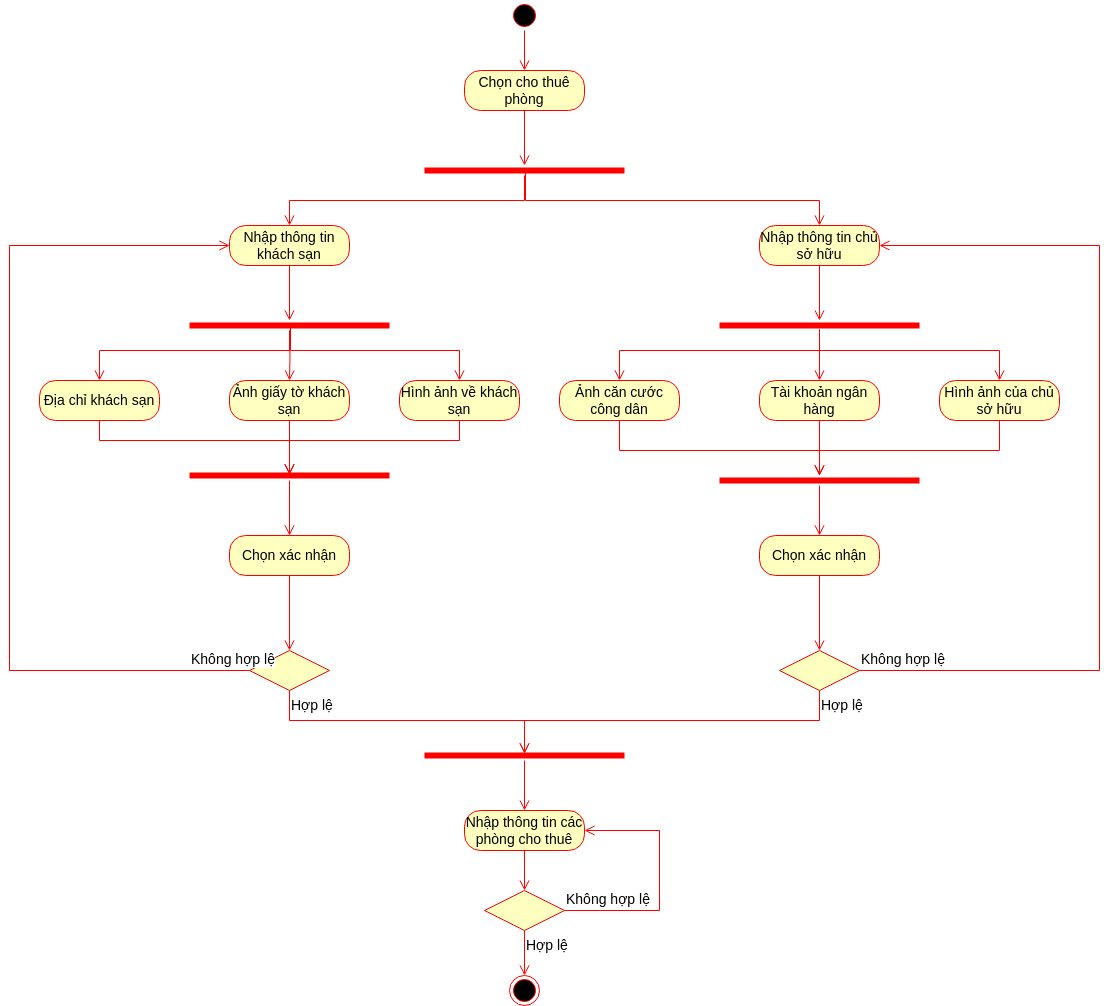
\includegraphics[width=\textwidth]{img/1.Việt-Cho thuê phòng.drawio.png}
    \caption{Biểu đồ hoạt động cho ca sử dụng Cho thuê phòng}
\end{figure}
\textbf{\indent Mô tả}\\
\indent Người dùng (chủ khách sạn hoặc người quản lý) thực hiện việc đăng ký khách sạn và phòng cho thuê trên hệ thống, hệ thống sẽ kiểm tra tính hợp lệ của thông tin trước khi xác nhận việc cho thuê phòng.

\textbf{Các tác nhân}\\
\indent Người dùng, authentication system.

\textbf{Điều kiện kích hoạt ca sử dụng}
\begin{itemize}
    \item Người dùng muốn đăng ký khách sạn và cho thuê phòng.
\end{itemize}

\textbf{Tiền điều kiện}
\begin{itemize}
    \item Người dùng phải có tài khoản hợp lệ để truy cập hệ thống.
    \item Hệ thống phải hoạt động bình thường.
    \item Người dùng phải có internet trong suốt thời gian hoạt động.
\end{itemize}

\textbf{Hậu điều kiện}
\begin{itemize}
    \item Nếu thông tin hợp lệ, phòng được đăng ký thành công trong hệ thống.
    \item Nếu thông tin không hợp lệ, hệ thống sẽ từ chối và yêu cầu chỉnh sửa.
\end{itemize}

\textbf{Các luồng sự kiện}

\begin{small}
\textbf{Luồng cơ bản}\\
\indent 1. Người dùng chọn cho thuê phòng\\
\indent 2. Người dùng nhập thông tin của cá nhân và khách sạn\\
\indent 3. Người dùng chọn xác nhận\\
\indent 4. Hệ thống kiểm tra các thông tin người dùng đã nhập\\
\indent 5. Người dùng nhập thông tin các phòng cho thuê\\
\indent 6. Hệ thống kiểm tra thông tin phòng.\\
\indent 7. Hiển thị thông báo thành công và kết thúc

\textbf{Luồng thay thế}\\
\indent 4.1 Thống báo thông tin không hợp lệ và quay lại bước 2\\
\indent 6.1 Hiển thị thông tin phòng không hợp lệ và quay lại bước 5\\
\end{small}\\
\textbf{\indent Business rules}
\begin{itemize}
    \item Thông tin khách khách sạn và chủ sở hữu phải đầy đủ chính xác.
    \item Ảnh CCCD và giấy tờ phải rõ ràng, không bị mờ.
    \item Tài khoản ngân hàng phải khớp với tên chủ sở hữu để tránh gian lận.
    \item Chỉ khi mọi thông tin hợp lệ thì phòng mới được đưa lên hệ thống.
\end{itemize}

\textbf{Yêu cầu phi chức năng}
\begin{itemize}
    \item Bảo mật: bảo vệ thông tin cá nhân của chủ khách sạn.
    \item Tích hợp: hệ thống có thể kết nối với ngân hàng để xác thực tài khoản.
\end{itemize}

\textbf{Extension point:} Không có



\subsection{Sửa thông tin phòng}
\begin{figure}[H]
    \centering
    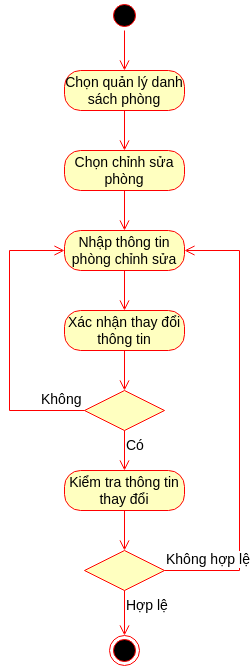
\includegraphics[width=0.4\textwidth]{img/1.Việt-Sửa thông tin phòng.drawio.png}
    \caption{Biểu đồ hoạt động cho ca sử dụng Sửa thông tin phòng}
\end{figure}
\textbf{\indent Mô tả}\\
\indent Hành động này cho phép người quản lý cập nhật thông tin của một phòng đã cho thuê trên ứng dụng.

\textbf{Các tác nhân}
\begin{itemize}
    \item \textbf{Người quản lý phòng:} tác nhân chính.
\end{itemize}
\textbf{Điều kiện kích hoạt ca sử dụng}
\begin{itemize}
    \item Người quản lý đã đăng nhập vào ứng dụng.
    \item Phòng cần cập nhật đã tồn tại trong hệ thống.
\end{itemize}

\textbf{Tiền điều kiện}
\begin{itemize}
    \item Phòng không ở trạng thái đang cho thuê.
    \item Tài khoản có phòng đã được đăng lên hệ thống.
\end{itemize}

\textbf{Hậu điều kiện}
\begin{itemize}
    \item Thông tin phòng được cập nhập nếu người dùng nhập đúng và hoàn tất kiểm tra.
    \item Thông tin phòng giữ nguyên nếu người dùng không xác nhận hoặc nhập thông tin không chính xác.
\end{itemize}

\textbf{Các luồng sự kiện}

\begin{small}
\textbf{Luồng cơ bản}\\
\indent 1. Người dùng chọn danh sách phòng đã cho thuê.\\
\indent 2. Chọn chỉnh sửa phòng muốn thay đổi.\\
\indent 3. Nhập những thông tin cần chỉnh sửa.\\
\indent 4. Người dùng xác nhận lưu thay đổi.\\
\indent 5. Hệ thống kiểm tra xác thực dữ liệu đầu vào.\\

\textbf{Luồng thay thế}\\
\indent 4.1 Nếu người quản lý nhấn "Hủy", hệ thống sẽ không lưu bất kỳ thay đổi nào.\\
\indent 5.1 Hiển thị thông báo thông tin phòng không hợp lệ, yêu cầu người dùng nhập lại thông tin phòng.
\end{small}\\
\textbf{\indent Business rules}
\begin{itemize}
    \item Thông tin phòng phải đầy đủ chính xác hình ảnh phải rõ nét.
    \item Chỉ khi mọi thông tin hợp lệ thì phòng mới được đưa lên hệ thống.
\end{itemize}

\textbf{Extension point:} Không có



\subsection{Tra cứu thông tin phòng đang cho thuê}
\begin{figure}[H]
    \centering
    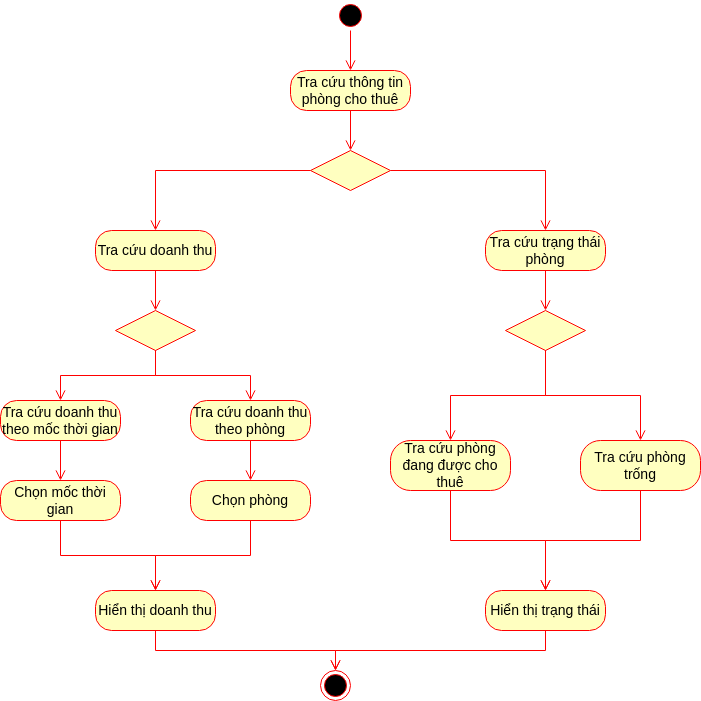
\includegraphics[width=\textwidth]{img/1.Việt-Tra cứu thông tin phòng đang cho thuê.drawio.png}
    \caption{Biểu đồ hoạt động cho ca sử dụng Tra cứu thông tin phòng đang cho thuê}
\end{figure}
\textbf{\indent Mô tả}
\begin{itemize}
    \item Doanh thu (theo khoảng thời gian hoặc theo phòng).
    \item Trạng thái các phòng (phòng đang được thuê hoặc phòng trống).
\end{itemize}

\textbf{Các tác nhân}
\begin{itemize}
    \item \textbf{Người quản lý phòng:} tác nhân chính.
\end{itemize}

\textbf{Điều kiện kích hoạt ca sử dụng}
\begin{itemize}
    \item Người dùng muốn xem thông tin về doanh thu hoặc tình trạng (trống/đang thuê) của phòng.
\end{itemize}

\textbf{Tiền điều kiện}
\begin{itemize}
    \item Người dùng đã đăng nhập hệ thống và có phòng cho thuê.
    \item Dữ liệu doanh thu và thông tin trạng thái phòng đã được hệ thống cập nhật.
\end{itemize}

\textbf{Hậu điều kiện}
\begin{itemize}
    \item Người dùng có được thông tin chính xác theo kết quả được tìm kiếm.
    \item Hệ thống hiển thị thông tin theo lựa chọn của người dùng.
\end{itemize}

\textbf{Các luồng sự kiện}

\begin{small}
\textbf{Luồng cơ bản}\\
\indent 1. Người dùng tra cứu thông tin phòng cho thuê\\
\indent 2. Người dùng chọn Tra cứu doanh thu hoặc Tra cứu trạng thái phòng\\
\indent 3. Người dụng chọn thông tin cần tra cứu\\
\indent 4. Hệ thống hiển thị thông tin

\textbf{Luồng thay thế}\\
\indent 3.1 Hệ thống không tìm kiếm được thời gian đã chọn, hiển thị thông báo không có thông tin về thời gian đã chọn.\\
\indent 3.2 Hệ thống không tìm kiếm được phòng đã chọn, hiển thị thông báo không có thông tin về phòng đã chọn.\\
\indent 3.3 Hệ thống không tìm thấy phòng còn trống, hiện thị thông báo không có phòng nào còn trống.\\
\indent 3.4 Hệ thống không tìm thấy phòng nào được thuê, hiển thị thông báo không có phòng nào được thuê.\\
\end{small}\\
\textbf{\indent Business rules}
\begin{itemize}
    \item Khoảng thời gian tra cứu phải hợp lệ (ví dụ: ngày bắt đầu trước ngày kết thúc).
    \item Thông tin về trạng thái phòng phải được cập nhật thường xuyên để đảm bảo tính chính xác.
    \item Người dùng chỉ xem được doanh thu nếu có quyền hạn phù hợp.
\end{itemize}

\textbf{Yêu cầu phi chức năng}
\begin{itemize}
    \item Hiệu suất: Hệ thống phải trả kết quả tra cứu doanh thu và trạng thái phòng nhanh
    \item Bảo mật: Chỉ những tài khoản có quyền xem doanh thu mới được phép xem báo cáo.
\end{itemize}

\textbf{Extension point}
\begin{itemize}
    \item Lọc nâng cao: Lọc trạng thái phòng theo nhiều tiêu chí (loại phòng, giá, vị trí...).
\end{itemize}



\subsection{Xóa phòng khách sạn}
\begin{figure}[H]
    \centering
    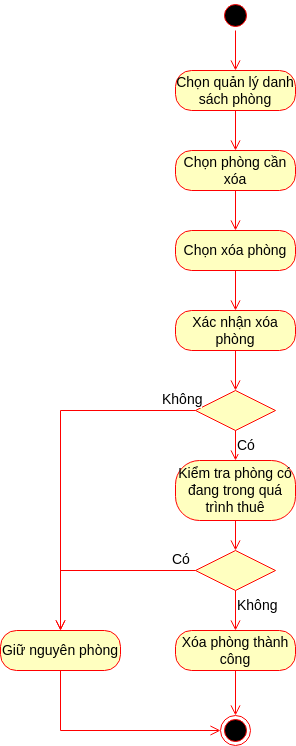
\includegraphics[width=0.5\textwidth]{img/1.Việt-Xóa phòng đang cho thuê.drawio.png}
    \caption{Biểu đồ hoạt động cho ca sử dụng Xóa phòng khách sạn}
\end{figure}
\textbf{\indent Mô tả}\\
\indent Hành động cho phép người quản lý phòng cho thuê xóa phòng của mình trên hệ thống.

\textbf{Các tác nhân}
\begin{itemize}
    \item \textbf{Người quản lý phòng:} tác nhân chính.
\end{itemize}

\textbf{Điều kiện kích hoạt ca sử dụng}
\begin{itemize}
    \item Người quản lý đã đăng nhập vào ứng dụng.
    \item Phòng cần cập nhật đã tồn tại trong hệ thống.
\end{itemize}

\textbf{Tiền điều kiện}
\begin{itemize}
    \item Tài khoản có phòng đã được đăng lên hệ thống.
\end{itemize}

\textbf{Hậu điều kiện}
\begin{itemize}
    \item Phòng sẽ được xóa nếu hoàn tất kiểm tra.
    \item Phòng sẽ không thay đổi nếu người dùng không xác nhận hoặc phòng đang trong quá trình thuê.
\end{itemize}

\textbf{Các luồng sự kiện}

\begin{small}
\textbf{Luồng cơ bản}\\
\indent 1. Người dùng chọn danh sách phòng đã cho thuê.\\
\indent 2. Chọn phòng muốn xóa.\\
\indent 3. Chọn nút xóa phòng.\\
\indent 4. Người dùng xác nhận xóa phòng.\\
\indent 5. Hệ thống kiểm tra phòng có đang trong quá trình thuê không.\\
\indent 6. Hệ thống thông báo xóa phòng thành công.\\

\textbf{Luồng thay thế}\\
\indent 4.1 Nếu người quản lý nhấn "Hủy", hệ thống sẽ không lưu bất kỳ thay đổi nào.\\
\indent 5.1 Hiển thị thông báo thông phòng đang trong quá trình thuê, yêu cầu người dùng xóa phòng khi không có khách thuê.\\
\end{small}\\
\textbf{\indent Business rules}: Không có.

\textbf{Yêu cầu phi chức năng:} Không có.

\textbf{Extension point:} Không có.

\subsection{Thanh toán}
\begin{figure}[H]
    \centering
    \includegraphics[width=0.5\textwidth]{img/1.5 Minh-Thanh toán.drawio.png}
    \caption{Biểu đồ hoạt động cho ca sử dụng Thanh toán}
\end{figure}
\textbf{\indent Mô tả}\\
\indent Người dùng thanh toán khoản tiền cần trả cho việc đặt phòng và tìm phương tiện (nếu có) bằng các hình thức khác nhau.

\textbf{Các tác nhân:} Người dùng, Ngân hàng.

\textbf{Điều kiện kích hoạt ca sử dụng}
\begin{itemize}
    \item Người dùng chọn chức năng thanh toán sau khi đặt phòng (hoặc đặt phương tiện).
\end{itemize}

\textbf{Tiền điều kiện}
\begin{itemize}
    \item Người dùng đã đăng nhập vào hệ thống.
    \item Thiết bị của người dùng kết nối Internet trong khi sử dụng dịch vụ.
    \item Người dùng đã đặt phòng (hoặc đặt phương tiện) và chọn mục thanh toán.
\end{itemize}

\textbf{Hậu điều kiện}
\begin{itemize}
    \item Thanh toán thành công: Hệ thống cập nhật lại trạng thái phòng và thông báo cho người dùng.
    \item Thanh toán thất bại: Hệ thống hiển thị thông báo lỗi.
\end{itemize}

\textbf{Các luồng sự kiện}

\begin{small}
\textbf{Luồng cơ bản}\\
\indent 1. Người dùng đặt phòng khách sạn (đặt phương tiện) và sau đó chọn mục thanh toán.\\
\indent 2. Hệ thống hiển thị thông tin dịch vụ và số tiền cần phải thanh toán.\\
\indent 3. Hệ thống hiển thị các phương thức thanh toán khả dụng.\\
\indent 4. Người dùng chọn 1 phương thức thanh toán phù hợp.\\
\indent 5. Người dùng nhập thông tin thanh toán.\\
\indent 6. Hệ thống xác nhận thông tin.\\
\indent 7. Hệ thống thông báo thanh toán thành công

\textbf{Luồng thay thế}\\
\indent 6.1 Hiển thị thông báo lỗi và quay lại bước 5\\
\end{small}\\
\textbf{\indent Business rules}
\begin{itemize}
    \item Hệ thống chỉ xác nhận đặt phòng thành công khi thanh toán được chấp nhận hoặc đặt cọc thành công.
    \item Nếu thanh toán thất bại, đặt phòng sẽ không được giữ cho đến khi người dùng hoàn tất giao dịch.
    \item Hệ thống phải tự động gửi email/SMS xác nhận sau khi thanh toán thành công.
    \item Người dùng có thể hủy phòng và nhận loại toàn bộ số tiền đã thanh toán.
    \item Hệ thống không lưu trữ trực tiếp thông tin thẻ tín dụng của khách hàng chỉ lưu mã token hóa do cổng thanh toán cung cấp.
    \item Hệ thống hỗ trợ 2FA (xác thực hai yếu tố).
    \item Nếu hệ thống báo thanh toán thành công nhưng đặt phòng không được xác nhận, hệ thống phải hoàn tiền trong vòng 3-5 ngày làm việc.
    \item Nếu giao dịch bị lỗi do hệ thống nhưng tiền đã bị trừ, hệ thống sẽ tự động xử lý hoàn tiền hoặc liên hệ hỗ trợ.
\end{itemize}

\textbf{Yêu cầu phi chức năng}
\begin{itemize}
    \item Hệ thống xử lý giao dịch trong vòng 5 giây để đảm bảo trải nghiệm mượt mà.
    \item Hỗ trợ nhiều giao dịch thanh toán đồng thời (hơn 1000) mà không bị gián đoạn.
    \item Hỗ trợ tất các cả trình duyệt phổ biến (Chrome, Safari, Firefox, …)
    \item Tương thích với Android, IOS.
\end{itemize}

\textbf{Extension point:} Mã giảm giá: Người dùng chọn mã giảm giá tại bước thanh toán, nếu mã hợp lệ thì hiển thị lại số tiền cần thanh toán, và nếu mã k hợp lệ thì hệ thộng hiển thị lỗi và yêu cầu nhập lại

\subsection{Tra cứu phương tiện}
\begin{figure}[H]
    \centering
    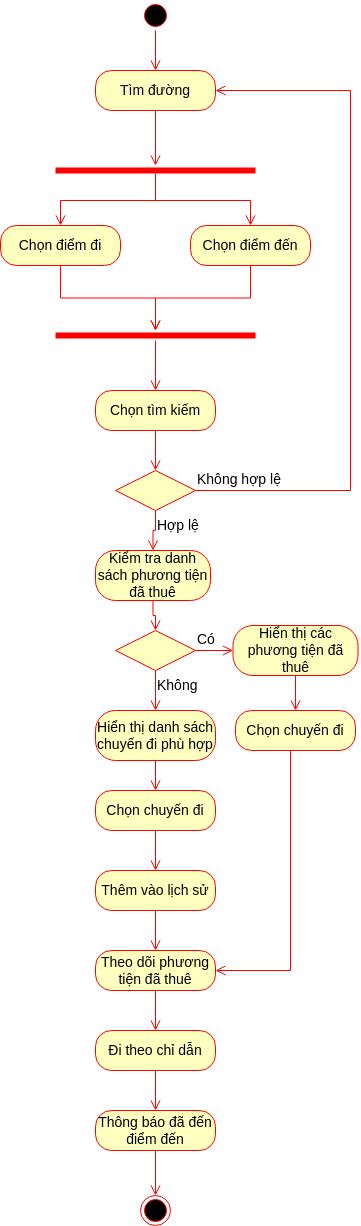
\includegraphics[width=0.39\textwidth]{img/1.5 Minh-Tìm phương tiện.drawio.png}
    \caption{Biểu đồ hoạt động cho ca sử dụng Tra cứu phương tiện}
\end{figure}
\textbf{\indent Mô tả}\\
\indent Người dùng sử dụng chức năng tìm phương tiện để được chỉ dẫn về các phương thức di chuyển từ vị trí hiện tại (hoặc một địa điểm cụ thể) đến khách sạn đã đặt (hoặc một địa điểm cụ thể). Hệ thống sẽ hiển thị các tùy chọn phương tiện phù hợp.

\textbf{Các tác nhân:} Người dùng, Google map.

\textbf{Điều kiện kích hoạt ca sử dụng}
\begin{itemize}
    \item Người dùng muốn tìm phương tiện để di chuyển đến khách sạn đã đặt.
\end{itemize}

\textbf{Tiền điều kiện}
\begin{itemize}
    \item Người dùng đã đặt phòng khách sạn thành công.
    \item Hệ thống hoạt động ổn định.
    \item Đảm bảo thiết bị có kết nối Internet.
\end{itemize}

\textbf{Hậu điều kiện}
\begin{itemize}
    \item Hệ thống hiển thị các phương tiện di chuyển từ điểm xuất phát đến khách sạn.
    \item Người dùng chọn phương tiện phù hợp và hệ thống sẽ hiển thị chi phí cần thanh toán.
    \item Hệ thống cập nhật trạng thái dịch vụ.
\end{itemize}

\textbf{Các luồng sự kiện}

\begin{small}
\textbf{Luồng cơ bản}\\
\indent 1. Ở giao diện chính của ứng dụng, sau khi đặt phòng thành công thì người dùng chọn mục Tìm phương tiện.\\
\indent 2. Người dùng chọn điểm xuất phát và điểm đến.\\
\indent 3. Sau đó chọn vào mục Tìm phương tiện và hệ thống sẽ hiển thị những phương tiện phù hợp cho người dùng dựa vào chi phí tốt nhất và thời gian di chuyển ngắn nhất.\\
\indent 4. Người dùng chọn phương tiện phù hợp với mình trong danh sách hiển thị, hệ thống hiển thị chi tiết thông tin chi tiết lộ trình và bản đồ theo dõi vị trí so với đường đi được chỉ dẫn.\\
\indent 5. Người dùng thanh toán chi phí và sử dụng dịch vụ.

\textbf{Luồng thay thế}\\
\indent 1.1 Người dùng mất kết nối Internet trong quá trình tìm kiếm phương tiện. Hệ thống sẽ hiển thị “Kết nối Internet bị gián đoạn. Vui lòng kiểm tra lại mạng và thử lại”. Hệ thống lưu trữ thông tin điểm đi/đến của người dùng để tiếp tục tìm kiếm ngay khi có lại kết nối.\\
\indent 2.1 Người dùng nhập điểm xuất phát không hợp lệ. Hệ thống sẽ hiển thị “Không tìm \\
\indent 3.1 Nếu hai điểm đến và đi quá gần nhau trong vòng 200m, hệ thống sẽ thông báo: "Hai điểm bạn chọn quá gần để sử dụng phương tiện". Hệ thống gợi ý tuyến đường đi bộ trên bản đồ.hoản không hợp lệ, Vui lòng kiểm tra lại”.\\
\end{small}\\
\textbf{\indent Business rules}
\begin{itemize}
    \item Hệ thống chỉ tìm kiếm phương tiện trong phạm vi khu vực có dịch vụ giao thông hỗ trợ.
    \item Nếu điểm đi hoặc điểm đến nằm ngoài khu vực hỗ trợ, hệ thống sẽ thông báo lỗi.
    \item Người dùng có thể lọc để sắp xếp lại thứ tự ưu tiên khi hiển thị kết quả.
    \item Hệ thống cung cấp thông tin về các loại phương tiện phù hợp
\end{itemize}

\textbf{Yêu cầu phi chức năng}
\begin{itemize}
    \item Hệ thống phải trả về kết quả tìm kiếm phương tiện trong vòng dưới 10 giây trong điều kiện mạng ổn định.
    \item Tốc độ hiển thị bản đồ và chỉ dẫn đường đi phải mượt mà, không bị giật lag.
    \item Hệ thống có thể xử lý đồng thời nhiều lượt tìm kiếm mà không ảnh hưởng đến hiệu suất.
    \item Dữ liệu vị trí của người dùng phải được mã hóa trước khi gửi lên server.
    \item Không chia sẻ dữ liệu vị trí cá nhân cho bên thứ ba nếu không có sự cho phép của người dùng.
\end{itemize}

\textbf{Extension point:} Không có.

\subsection{Đăng ký tài khoản}
\begin{figure}[H]
    \centering
    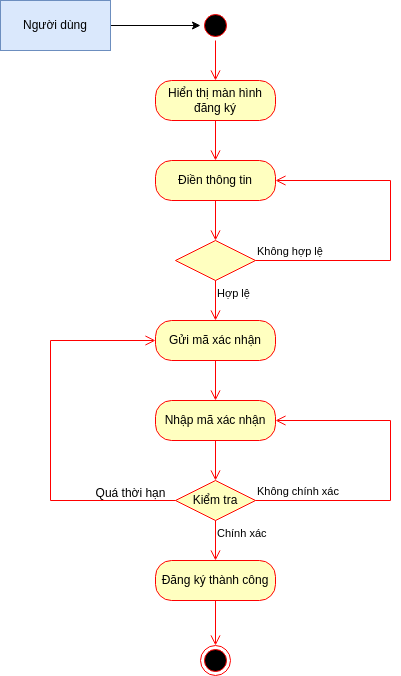
\includegraphics[width=0.65\textwidth]{img/Activity_graph-Đăng kí.drawio.png}
    \caption{Biểu đồ hoạt động cho ca sử dụng Đăng ký tài khoản}
\end{figure}
\textbf{\indent Mô tả}\\
\indent Người dùng khai báo thông tin để tạo tài khoản và truy cập đầy đủ các chức năng của hệ thống.

\textbf{Các tác nhân:} Người dùng.

\textbf{Điều kiện kích hoạt ca sử dụng}
\begin{itemize}
    \item Người dùng chọn chức năng đăng ký tài khoản.
\end{itemize}

\textbf{Tiền điều kiện}
\begin{itemize}
    \item Người dùng muốn tạo tài khoản.
    \item Người dùng có đầy đủ thông tin mà hệ thống yêu cầu.
    \item Thiết bị của người dùng được kết nối internet trong suốt ca sử dụng.
\end{itemize}

\textbf{Hậu điều kiện}
\begin{itemize}
    \item Người dùng đăng ký tài khoản thành công
\end{itemize}

\textbf{Các luồng sự kiện}

\begin{small}
\textbf{Luồng cơ bản}\\
\indent 1. Người dùng truy cập vào ứng dụng.\\
\indent 2. Người dùng chọn chức năng đăng ký tài khoản.\\
\indent 3. Hệ thống cung cấp form điền thông tin đăng ký tài khoản.\\
\indent 4. Người dùng điền thông tin đầy đủ vào các trường dữ liệu trong form đăng ký.\\
\indent 5. Hệ thống xác nhận tính hợp lệ của thông tin mà người dùng điền vào form.\\
\indent 6. Hệ thống gửi đường dẫn mã xác nhận kích hoạt tài khoản bằng tin nhắn đến.\\
\indent 7. Người dùng nhập mã xác nhận kích hoạt tài khoản.\\
\indent 8. Hệ thống kiểm tra mã xác nhận.\\
\indent 9. Hệ thống hiển thị thông báo đăng ký thành công.\\
\indent 10.Kết thúc ca sử dụng.\\

\textbf{Luồng thay thế}\\
\indent 5.1 Hiển thị thông báo thông tin không hợp lệ và quay lại bước 4.\\
\indent 8.1 Hiển thị thông báo mã xác nhận không chính xác và quay lại bước 7.\\
\indent 8.2 Hiển thị thông báo mã xác nhận đã quá hạn và quay lại bước 6.\\
\end{small}\\
\textbf{\indent Business rules:} Không có

\textbf{Yêu cầu phi chức năng}: Không có

\textbf{Extension point}: Không có

\subsection{Đăng nhập}
\begin{figure}[H]
    \centering
    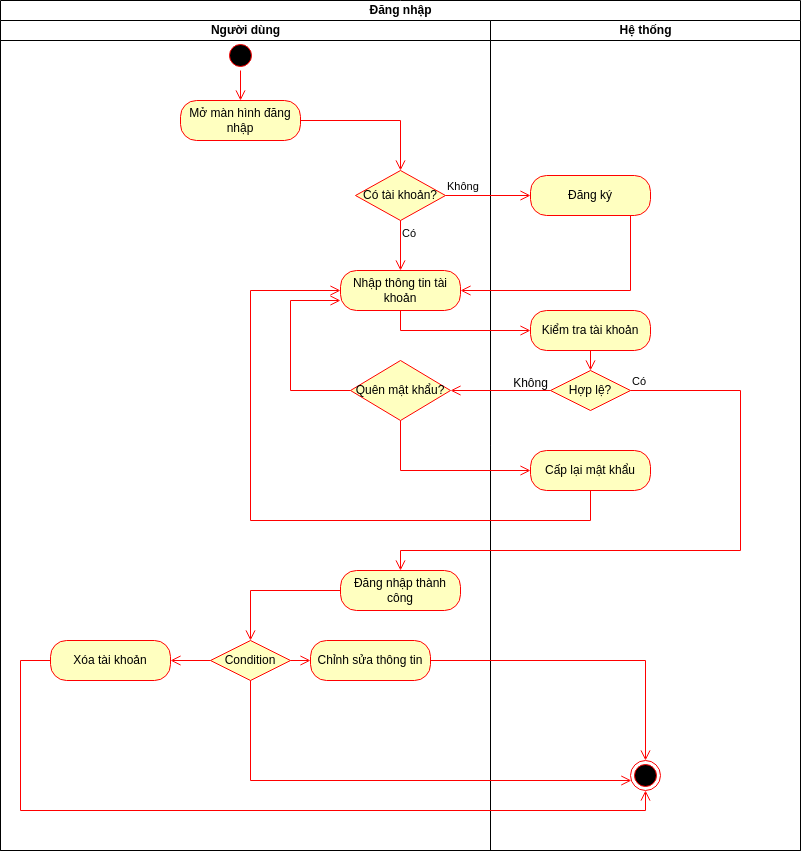
\includegraphics[width=0.9\textwidth]{img/Activity_graph-Đăng nhập.drawio.png}
    \caption{Biểu đồ hoạt động cho ca sử dụng Đăng nhập}
\end{figure}
\textbf{\indent Mô tả}\\
\indent Người dùng xác minh danh tính của mình để đăng nhập sử dụng hệ thống và chỉnh sửa tài khoản.

\textbf{Các tác nhân:} Người dùng, Cơ sở dữ liệu người dùng.

\textbf{Điều kiện kích hoạt ca sử dụng}
\begin{itemize}
    \item Người dùng chọn chức năng đăng nhập tài khoản
\end{itemize}

\textbf{Tiền điều kiện}
\begin{itemize}
    \item Hệ thống hiển thị giao diện đăng nhập ở trạng thái chờ
    \item Thiết bị của người dùng được kết nối internet trong suốt ca sử dụng
\end{itemize}

\textbf{Hậu điều kiện:} Không có

\textbf{Các luồng sự kiện}

\begin{small}
\textbf{Luồng cơ bản}\\
\indent 1. Người dùng truy cập vào ứng dụng.\\
\indent 2. Người dùng chọn chức năng đăng nhập.\\
\indent 3. Nếu người dùng có tài khoản, hệ thống cung cấp form điền thông tin đăng nhập tài khoản.\\
\indent 4. Người dùng điền số điện thoại và mật khẩu vào form đăng nhập.\\
\indent 5. Hệ thống xác minh thông tin của người dùng.\\
\indent 6. Hệ thống hiển thị đăng nhập thành công.\\
\indent 7. Kết thúc ca sử dụng\\

\textbf{Luồng thay thế}\\
\indent 3.1 Người dùng không có tài khoản có thể chuyển sang chức năng đăng ký.\\
\indent 5.1 Người dùng chọn quên mật khẩu.\\
\indent 5.2 Hiển thị thông báo thông tin bị sai và yêu cầu người dùng nhập lại tài khoản, mật khẩu.\\
\indent 6.1 Người dùng chọn chỉnh sửa thông tin sau đó kết thúc ca sử dụng.\\
\indent 6.2 Người dùng chọn xóa tài khoản sau đó kết thúc ca sử dụng.\\
\end{small}\\
\textbf{\indent Business rules:} Không có

\textbf{Yêu cầu phi chức năng}: Không có

\textbf{Extension point}:

\begin{small}
\textbf{Lấy lại mật khẩu:}\\
\indent 5.1.1 Người dùng chọn chức năng quên mật khẩu.\\
\indent 5.1.2 Hệ thống yêu cầu người dùng nhập số điện thoại để xác minh tài khoản.\\
\indent 5.1.3 Người dùng nhập số điện thoại vào trường dữ liệu hệ thống hiển thị.\\
\indent 5.1.4a Hệ thống xác nhận tài khoản trùng khớp với số điện thoại và yêu cầu nhập mật khẩu mới.\\
\indent 5.1.4b Nếu tài khoản không tồn tại, hệ thống báo lỗi.\\
\indent 5.1.5 Người dùng nhập mật khẩu mới và bấm tiếp tục.\\
\indent 5.1.6 Hệ thống thông báo tạo mật khẩu mới thành công.\\

\textbf{Chỉnh sửa thông tin hồ sơ}\\
\indent 6.1.1 Tại giao diện chính, người dùng chọn chức năng thay đổi thông tin.\\
\indent 6.1.2 Hệ thống hiển thị form dữ liệu mà người dùng cung cấp khi đăng ký tài khoản.\\
\indent 6.1.3 Người dùng thay đổi thông tin trên các trường dữ liệu cần đổi và bấm hoàn thành.\\
\indent 6.1.4 Hệ thống hiển thị thông báo xác nhận thay đổi thông tin thành công.\\

\textbf{Xóa tài khoản}\\
\indent 6.2.1 Tại giao diện chính, người dùng chọn chức năng xóa tài khoản.\\
\indent 6.2.2 Hệ thống hiển thị thông báo xác nhận yêu cầu xóa tài khoản.\\
\indent 6.2.3 Người dùng bấm chọn xác nhận lại yêu cầu.\\
\indent 6.2.4 Hệ thống xóa dữ liệu tài khoản người dùng.\\
\end{small}\\


\subsection{Lựa chọn ngôn ngữ}
\begin{figure}[H]
    \centering
    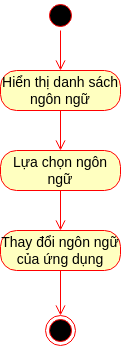
\includegraphics[width=0.2\textwidth]{img/Activity_graph-Lựa chọn ngôn ngữ.drawio.png}
    \caption{Biểu đồ hoạt động cho ca sử dụng Lựa chọn ngôn ngữ}
\end{figure}
\textbf{\indent Mô tả}\\
\indent Người dùng chọn ngôn ngữ phù hợp với bản thân.

\textbf{Các tác nhân}\\
\indent Người dùng

\textbf{Điều kiện kích hoạt ca sử dụng}
\begin{itemize}
    \item Người dùng lần đầu truy cập hệ thống.
\end{itemize}

\textbf{Tiền điều kiện}
\begin{itemize}
    \item Người dùng truy cập hệ thống.
\end{itemize}

\textbf{Hậu điều kiện}
\begin{itemize}
    \item Người dùng chọn ngôn ngữ thành công.
    \item Hệ thống lưu lại lựa chọn và thay đổi ngôn ngữ tương ứng.
\end{itemize}

\textbf{Các luồng sự kiện}

\begin{small}
\textbf{Luồng cơ bản}\\
\indent 1. Hệ thống đưa lựa chọn ngôn ngữ.\\
\indent 2. Người dùng chọn ngôn ngữ tương ứng.\\
\indent 3. Hiển thị thông báo thay đổi thành công và kết thúc ca sử dụng.\\
\end{small}\\
\textbf{\indent Business rules:} Không có.

\textbf{Yêu cầu phi chức năng: }Không có

\textbf{Extension point:} Không có.


\chapter{Phân tích hệ thống}
\section{Phân tích kiến trúc}
\subsection{Key abstraction}
\begin{figure}[H]
    \centering
    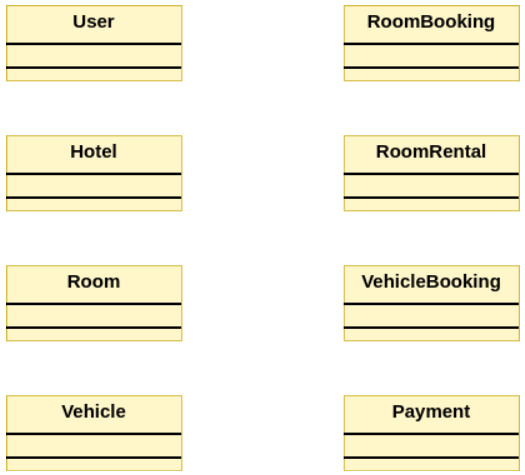
\includegraphics[width=0.6\textwidth]{img2/Key abstraction.png} 
    \caption{Danh sách Key abstraction}
\end{figure}

\textbf{\indent User}
\begin{itemize}
    \item Định nghĩa: Là tài khoản của người dùng để thực hiện các chức năng như thuê phòng, thuê phương tiện và cho thuê phòng
    \item Cơ chế phân tích: Persistency, Security
\end{itemize}

\textbf{Hotel}
\begin{itemize}
    \item Định nghĩa: là đối tượng chứa thông tin về các phòng và dịch vụ.
    \item Cơ chế phân tích: Persistency
\end{itemize}

\textbf{Room}
\begin{itemize}
    \item Định nghĩa: là đối tượng đại diện cho các phòng có thể được thuê của một khách sạn.
    \item Cơ chế phân tích: Persistency
\end{itemize}

\textbf{Vehicle}
\begin{itemize}
    \item Định nghĩa: là đối tượng đại diện cho các phương tiện có thể được thuê.
    \item Cơ chế phân tích: Persistency
\end{itemize}

\textbf{RoomBooking}
\begin{itemize}
    \item Định nghĩa: là đối tượng quản lý việc đặt phòng của người dùng.
    \item Cơ chế phân tích: Persistency
\end{itemize}

\textbf{RoomRental}
\begin{itemize}
    \item Định nghĩa: là đối tượng quản lý việc cho thuê phòng trọ của người dùng.
    \item Cơ chế phân tích: Persistency
\end{itemize}

\textbf{VehicleBooking}
\begin{itemize}
    \item Định nghĩa: là đối tượng quản lý việc đặt phương tiện của người dùng.
    \item Cơ chế phân tích: Persistency
\end{itemize}

\textbf{Payment}
\begin{itemize}
    \item Định nghĩa: là đối tượng quản lý việc thanh toán của người dùng.
    \item Cơ chế phân tích: Persistency, Security
\end{itemize}
\subsection{Thành phần cấp cao và sự phụ thuộc}
\begin{figure}[H]
    \centering
    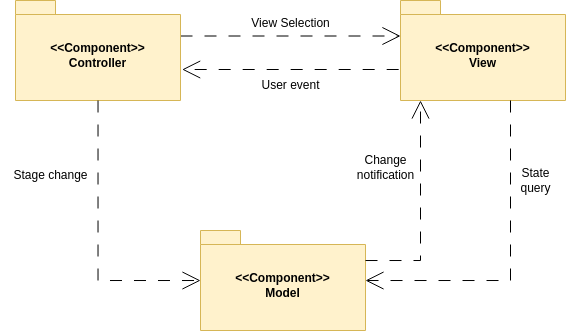
\includegraphics[width=0.8\textwidth]{img2/MVC.drawio.png} 
    \caption{Mô hình MVC}
\end{figure}
\begin{itemize}
    \item \textbf{Controller:} 	Điều phối luồng xử lý giữa View và Model
    \item \textbf{Model:} Tính toán nghiệp vụ, xử lý và kiểm tra dữ liệu
    \item \textbf{View:} hiển thị thông tin, tương tác trực tiếp với người dùng, chuyển tiếp các yêu cầu tới hệ thống và hiển thị kết quả đầu ra cho người dùng.
\end{itemize}

\section{Phân tích Use case}
\subsection{Biểu đồ tuần tự các use case}
\subsubsection{Đặt phòng khách sạn}
\begin{figure}[H]
    \centering
    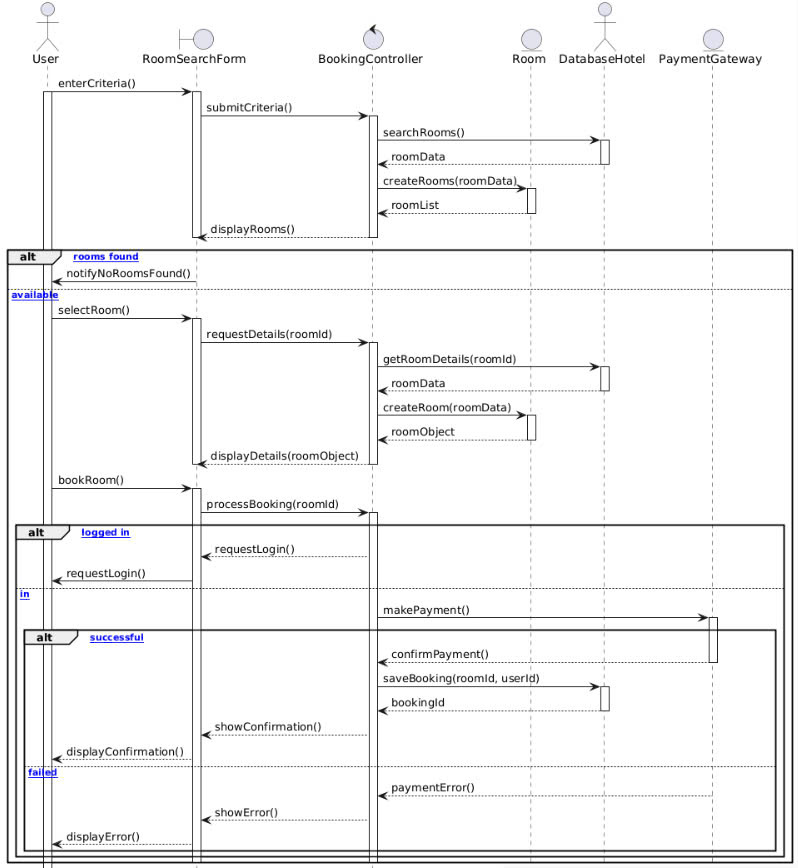
\includegraphics[width=\textwidth]{img2/timthue.jpg}
    \caption{Biểu đồ tuần tự ca sử dụng Đặt phòng khách sạn}
\end{figure}

\subsubsection{Theo dõi phòng đã đặt}
\begin{figure}[H]
    \centering
    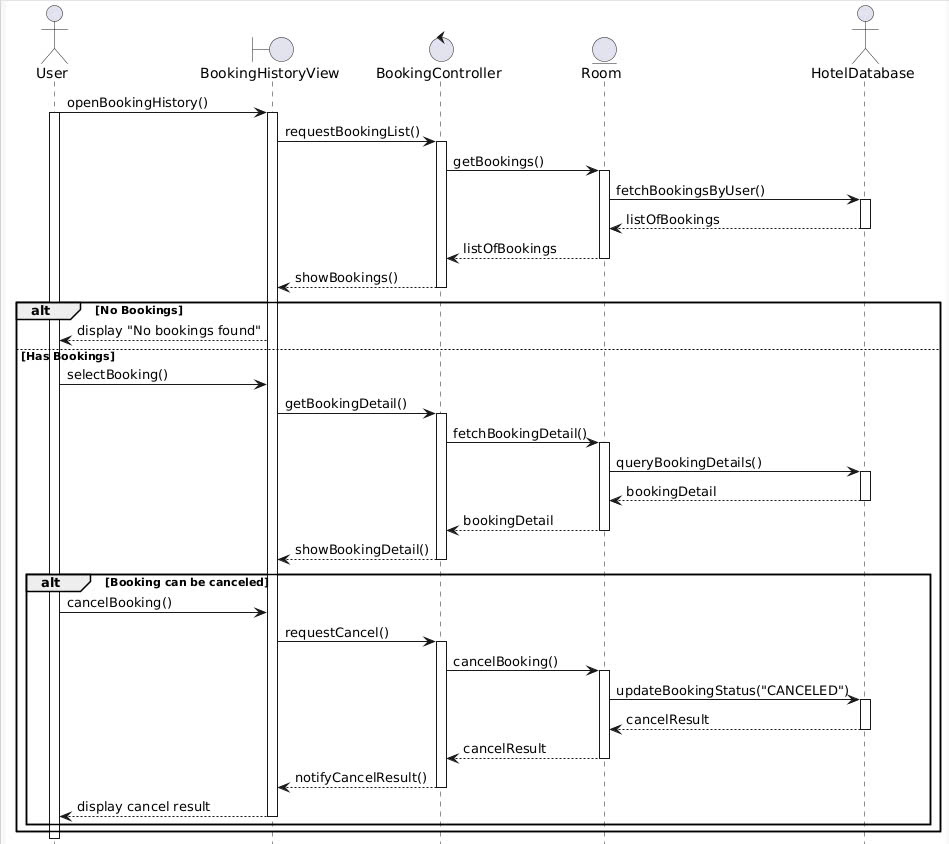
\includegraphics[width=\textwidth]{img2/xemphongdathue.jpg}
    \caption{Biểu đồ tuần tự ca sử dụng Theo dõi phòng đã đặt}
\end{figure}

\subsubsection{Đánh giá phòng đã thuê}
\begin{figure}[H]
    \centering
    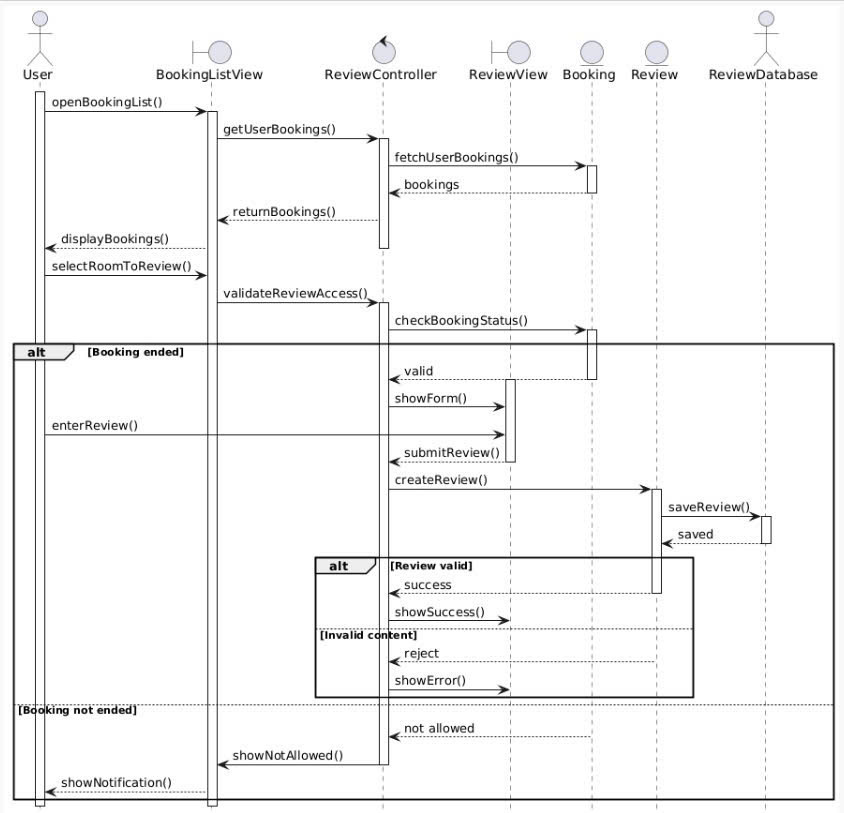
\includegraphics[width=\textwidth]{img2/danhgia.jpg}
    \caption{Biểu đồ tuần tự ca sử dụng Đánh giá phòng đã thuê}
\end{figure}

\subsubsection{Liên hệ với chủ khách sạn}
\begin{figure}[H]
    \centering
    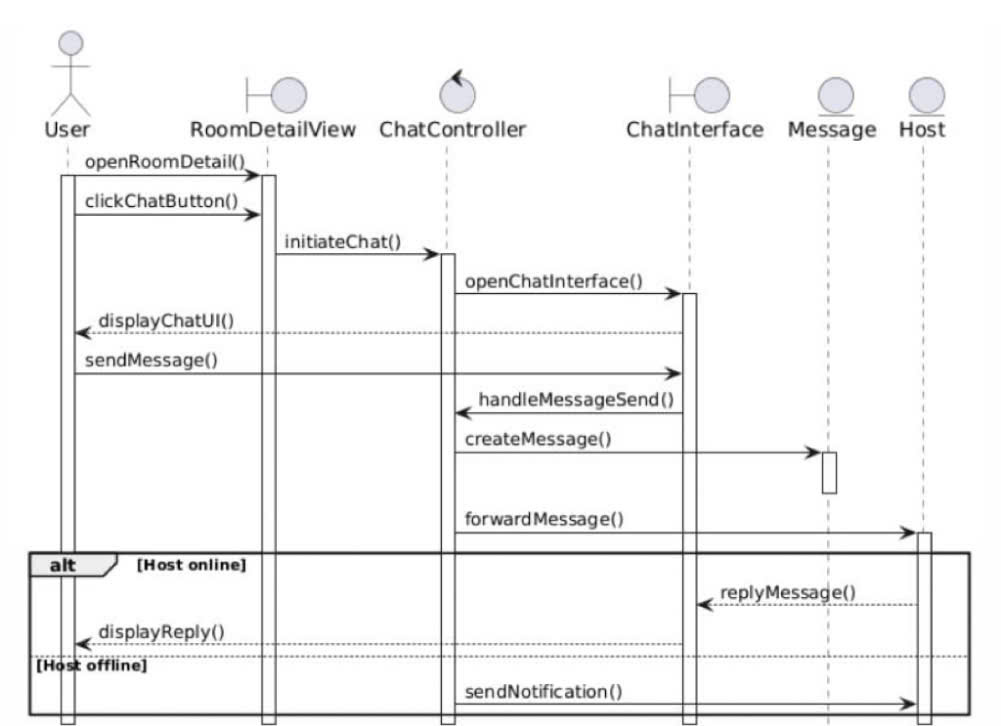
\includegraphics[width=\textwidth]{img2/chat.jpg}
    \caption{Biểu đồ tuần tự ca sử dụng Liên hệ với chủ khách sạn}
\end{figure}

\subsubsection{Xem danh sách phòng yêu thích}
\begin{figure}[H]
    \centering
    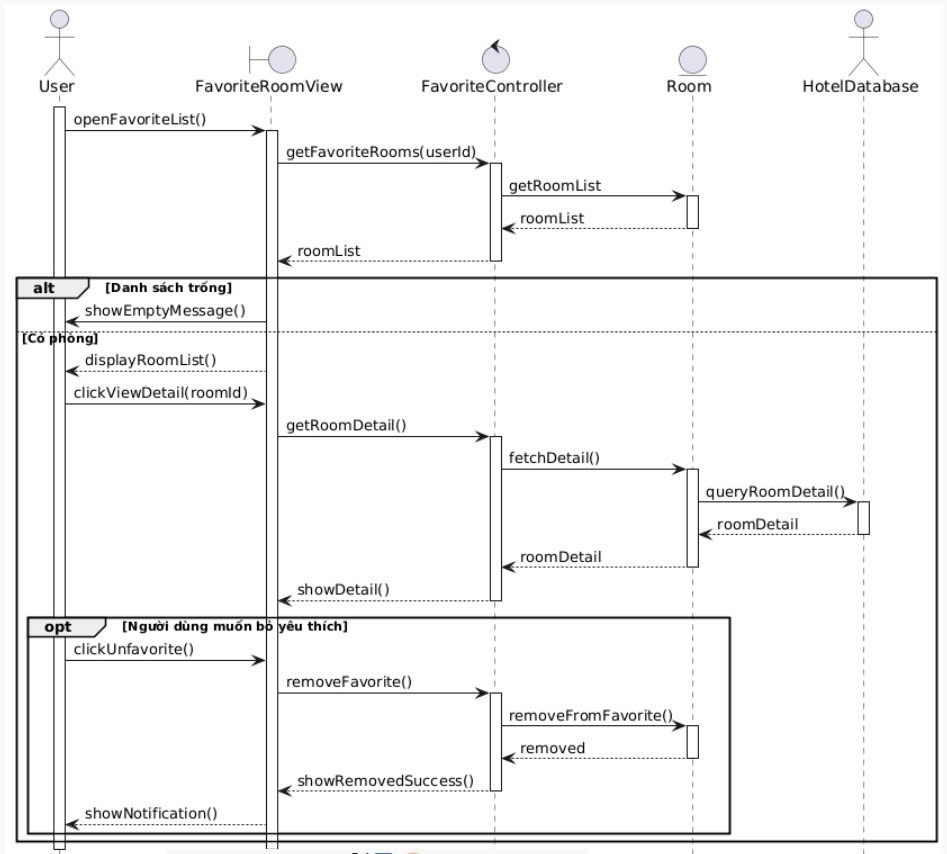
\includegraphics[width=\textwidth]{img2/xemphongyeuthich.jpg}
    \caption{Biểu đồ tuần tự ca sử dụng Xem danh sách phòng yêu thích}
\end{figure}

\subsubsection{Cho thuê phòng}
\begin{figure}[H]
    \centering
    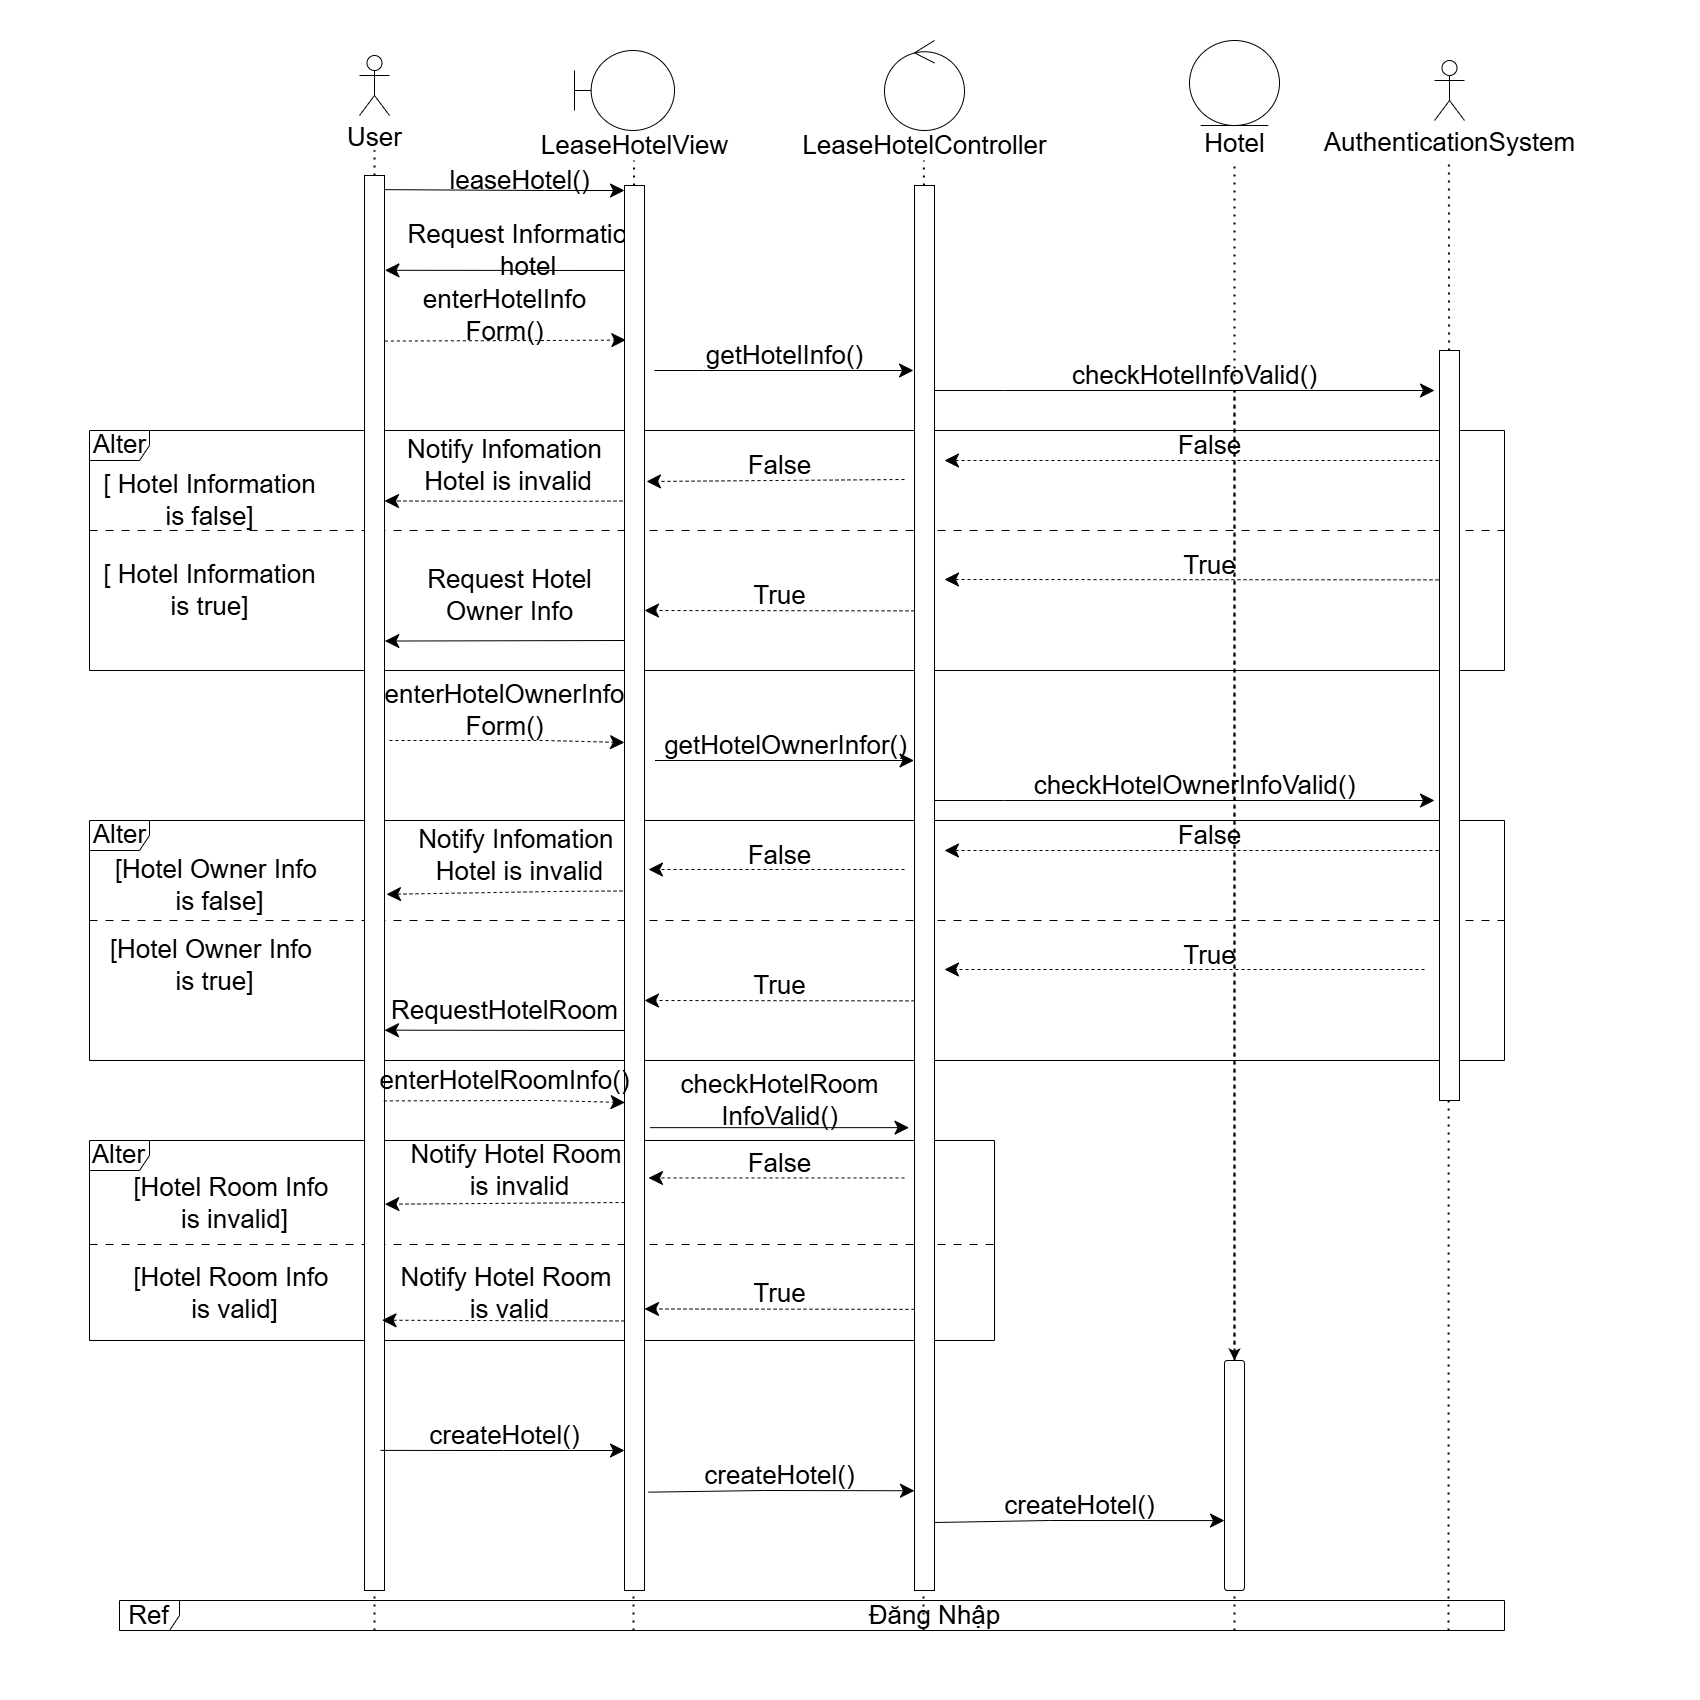
\includegraphics[width=\textwidth]{img2/chothuephong.png}
    \caption{Biểu đồ tuần tự ca sử dụng Cho thuê phòng}
\end{figure}

\subsubsection{Chỉnh sửa thông tin phòng khách sạn}
\begin{figure}[H]
    \centering
    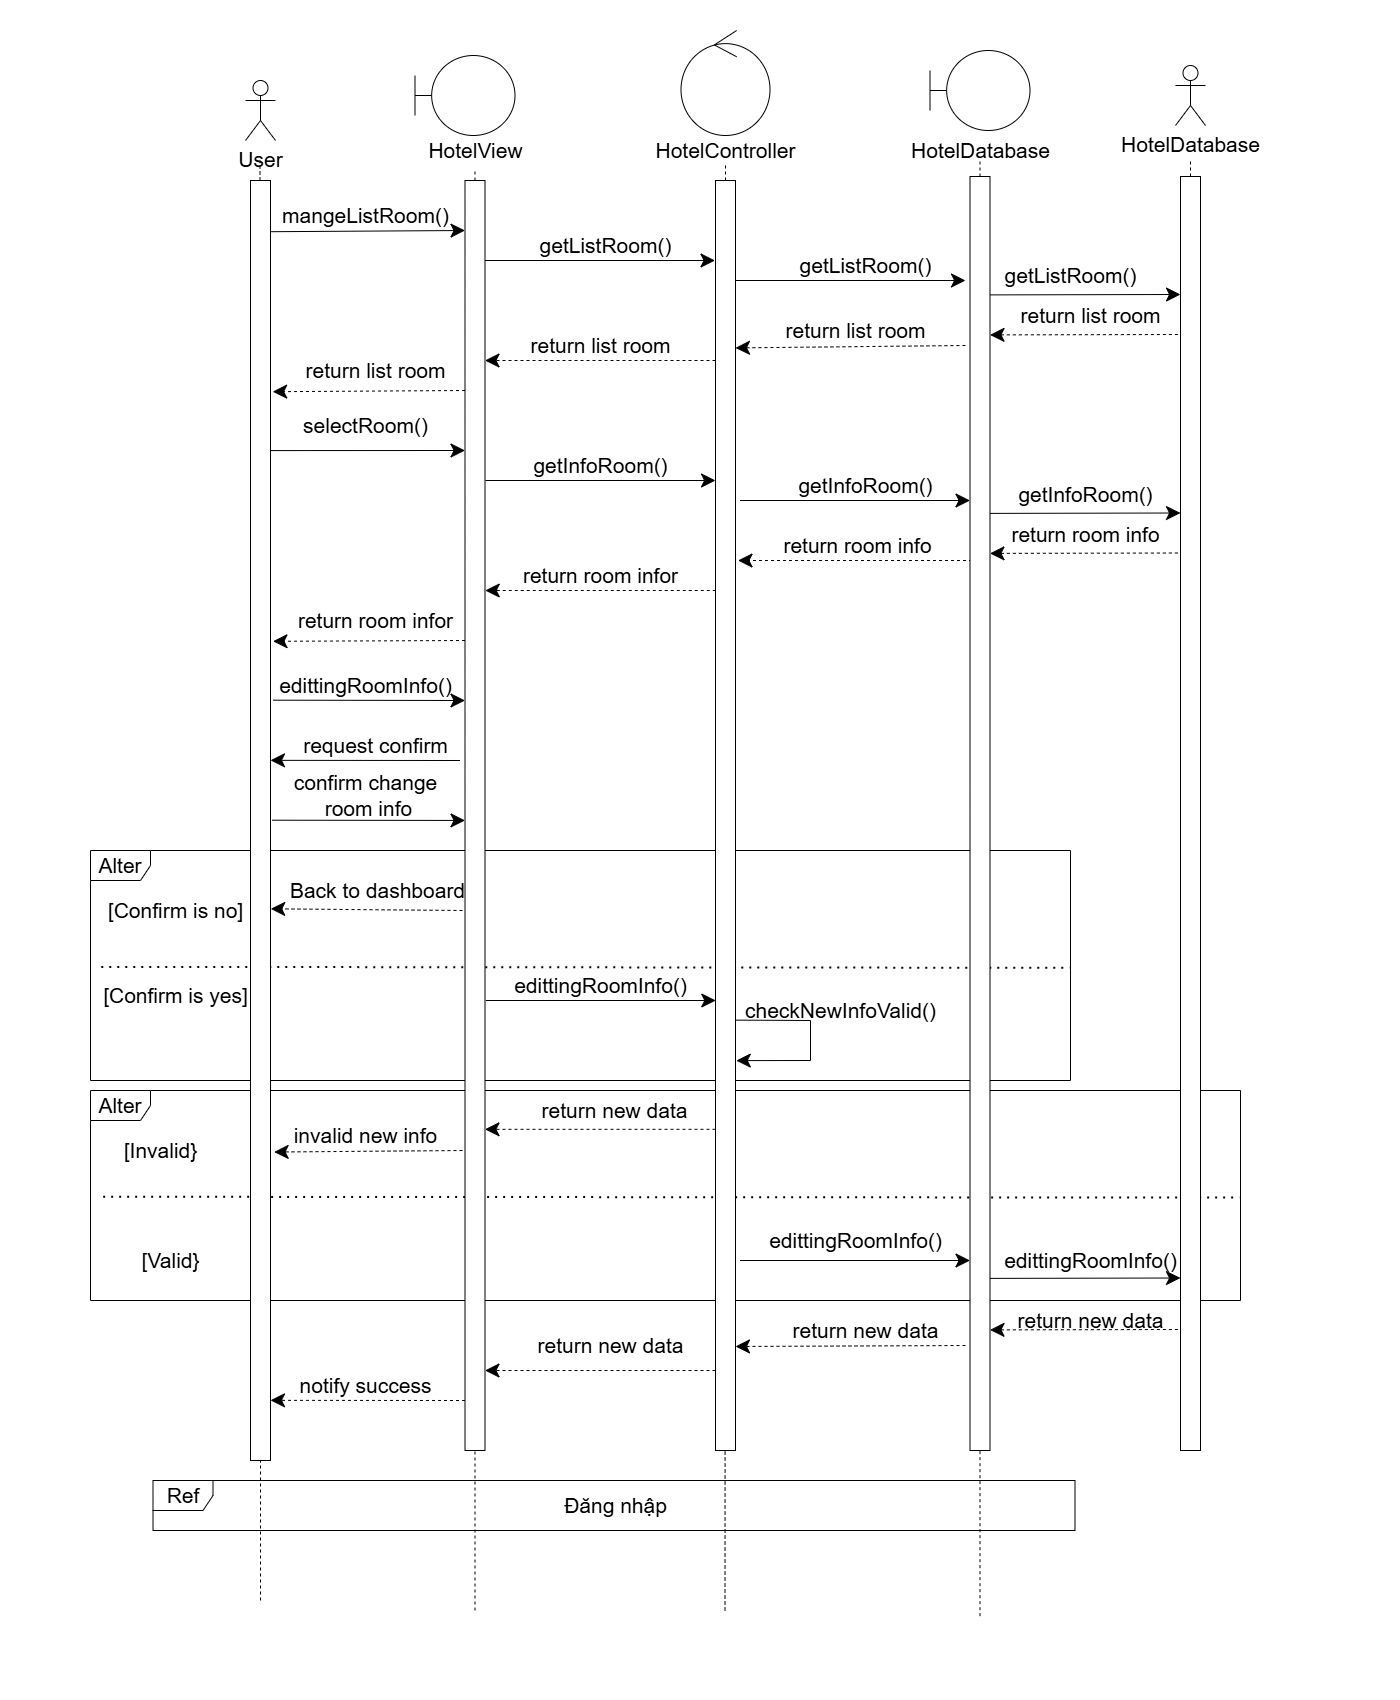
\includegraphics[width=\textwidth]{img2/chinhsuathongtinpt.png}
    \caption{Biểu đồ tuần tự ca sử dụng Chỉnh sửa thông tin phòng khách sạn}
\end{figure}

\subsubsection{Tra cứu thông tin phòng cho thuê}
\begin{figure}[H]
    \centering
    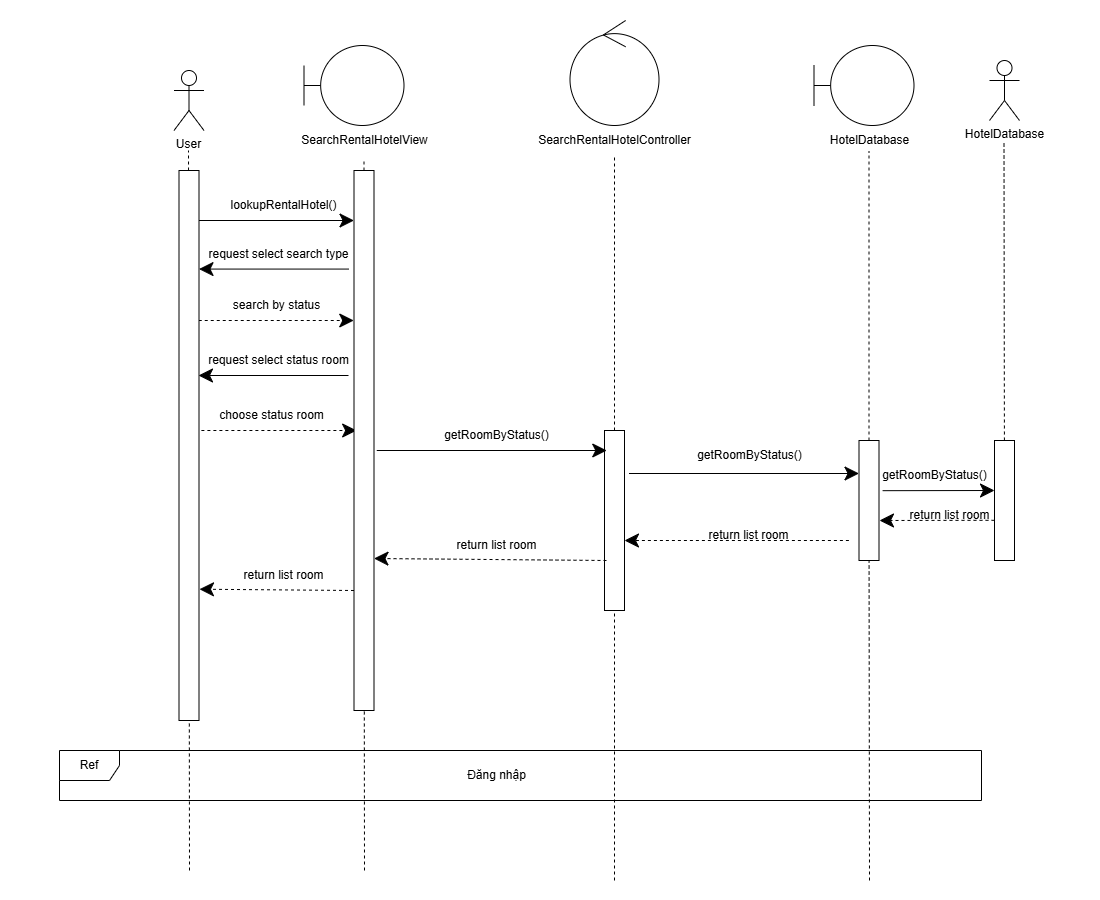
\includegraphics[width=\textwidth]{img2/tracuutrangthaiphongpt.png}
    \caption{Biểu đồ tuần tự ca sử dụng Tra cứu phòng cho thuê theo status}
\end{figure}

\begin{figure}[H]
    \centering
    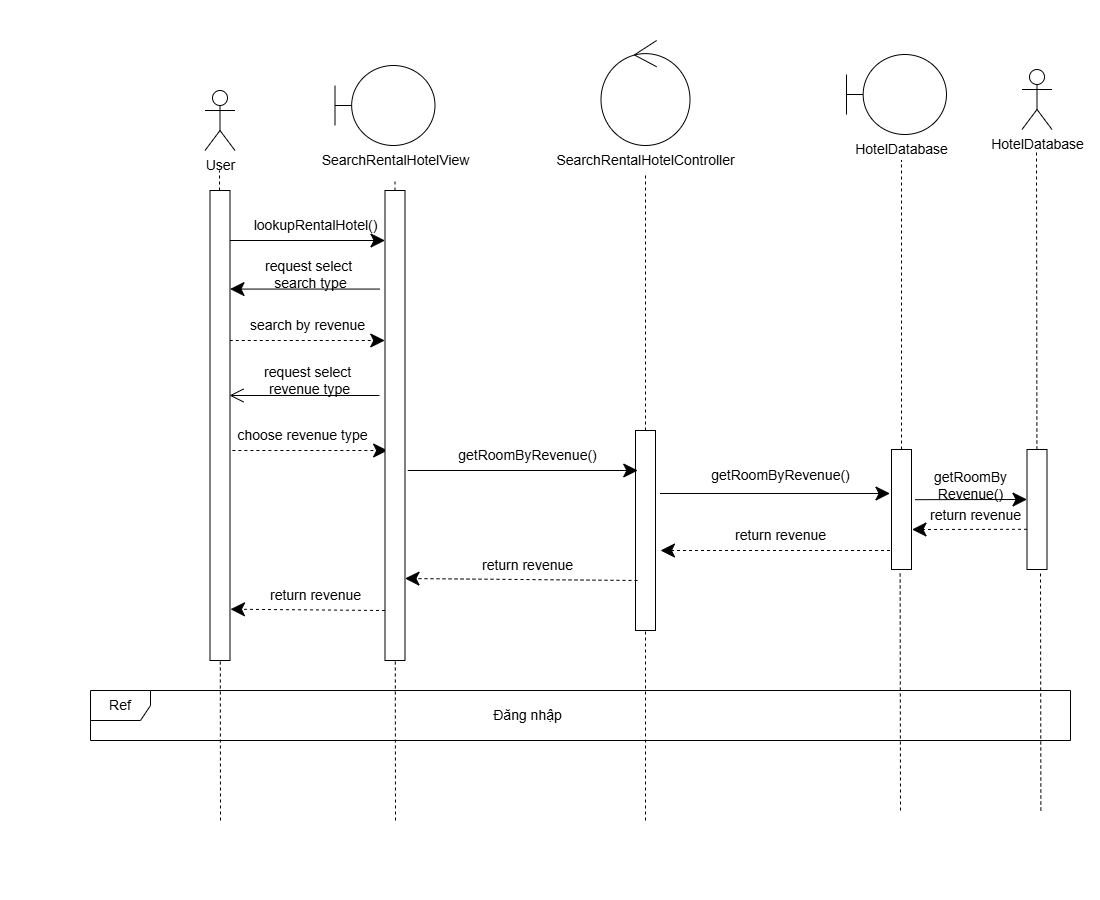
\includegraphics[width=\textwidth]{img2/tracuutheodoanhthupt.png}
    \caption{Biểu đồ tuần tự ca sử dụng Tra cứu phòng cho thuê theo revenue}
\end{figure}

\subsubsection{Xóa phòng khách sạn}
\begin{figure}[H]
    \centering
    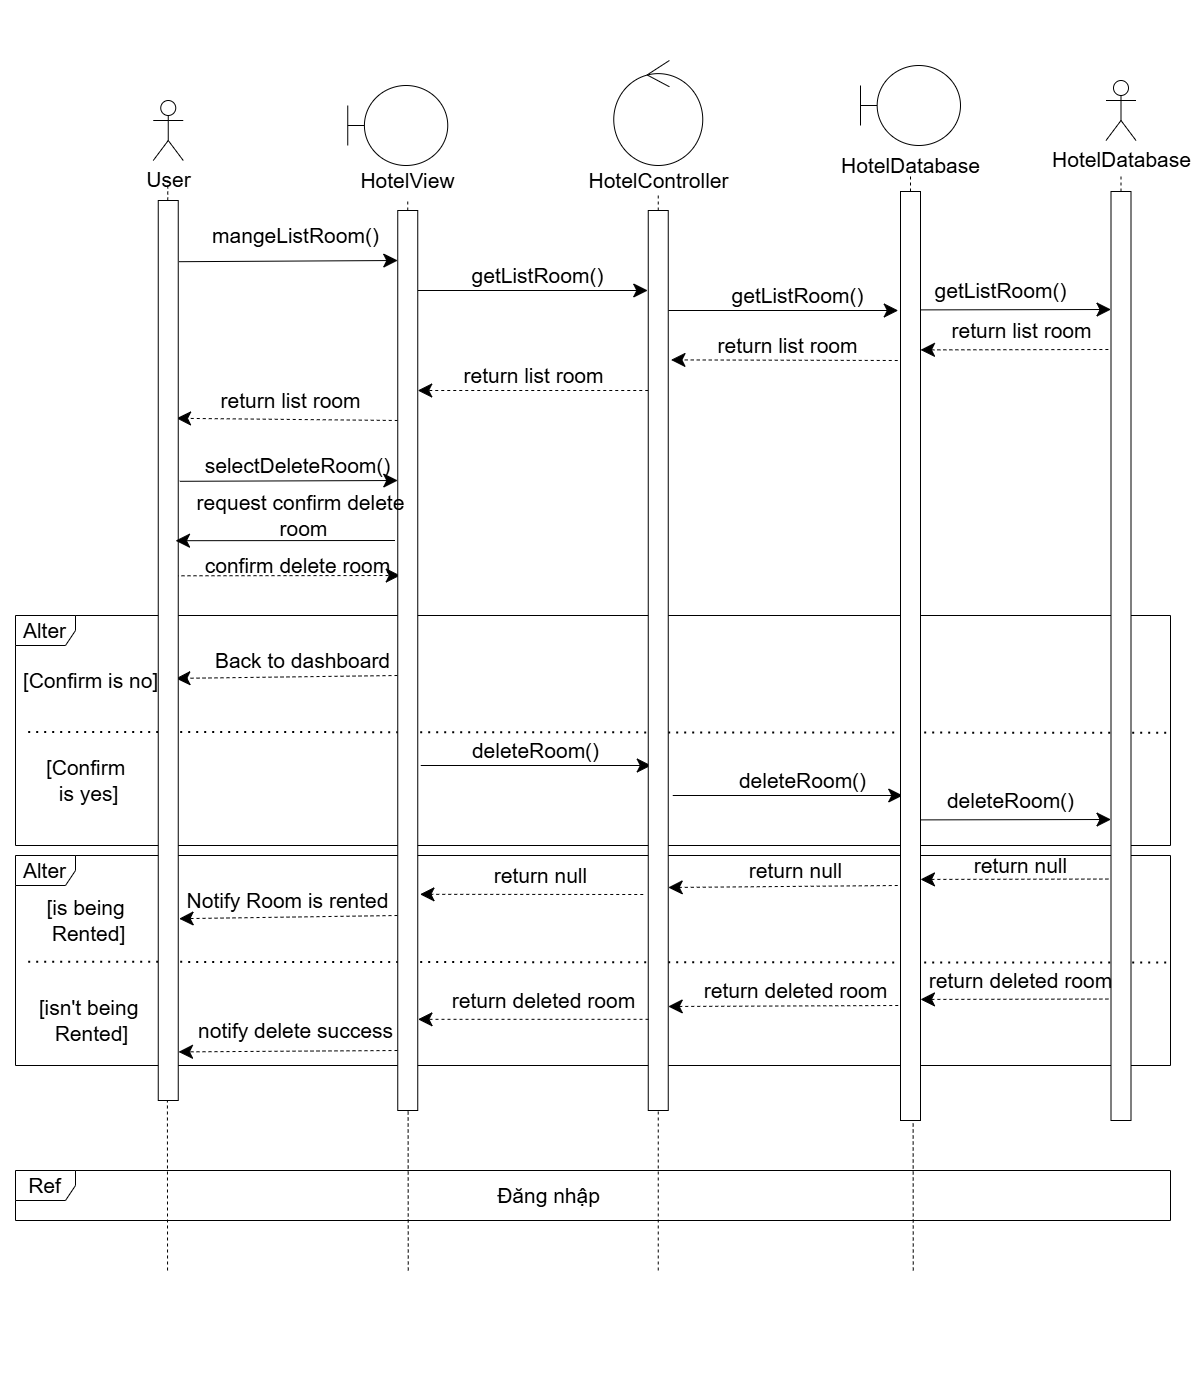
\includegraphics[width=\textwidth]{img2/xoaphongpt.png}
    \caption{Biểu đồ tuần tự ca sử dụng Xóa phòng khách sạn}
\end{figure}

\subsubsection{Thanh toán}
\begin{figure}[H]
    \centering
    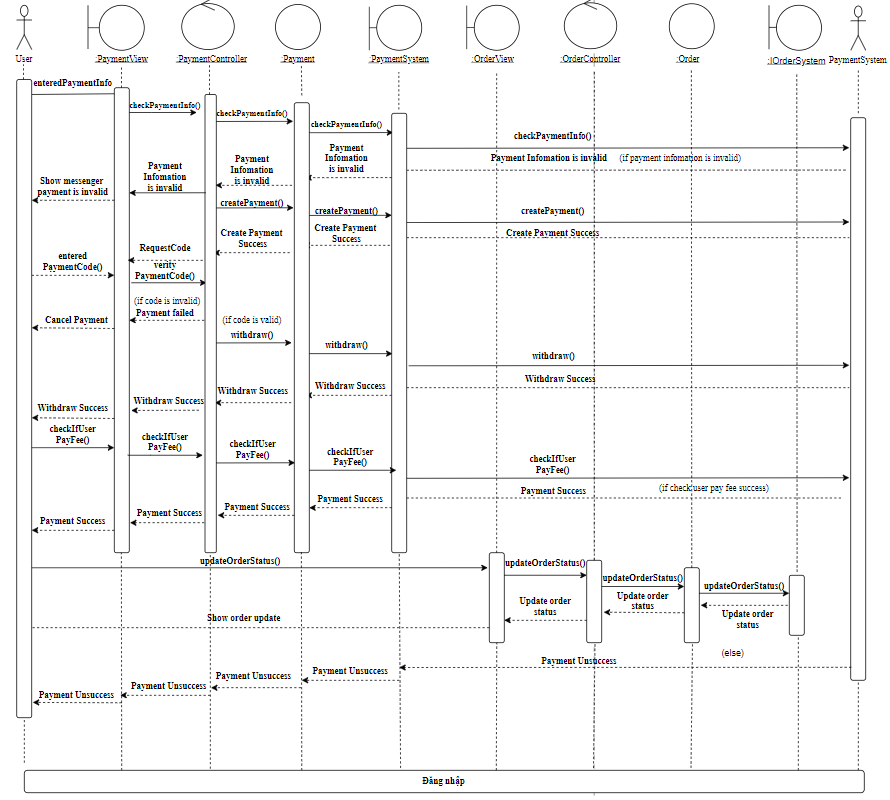
\includegraphics[width=\textwidth]{img2/2.1thanhtoanbangtk.png}
    \caption{Biểu đồ tuần tự ca sử dụng Thanh toán trực tuyến}
\end{figure}

\begin{figure}[H]
    \centering
    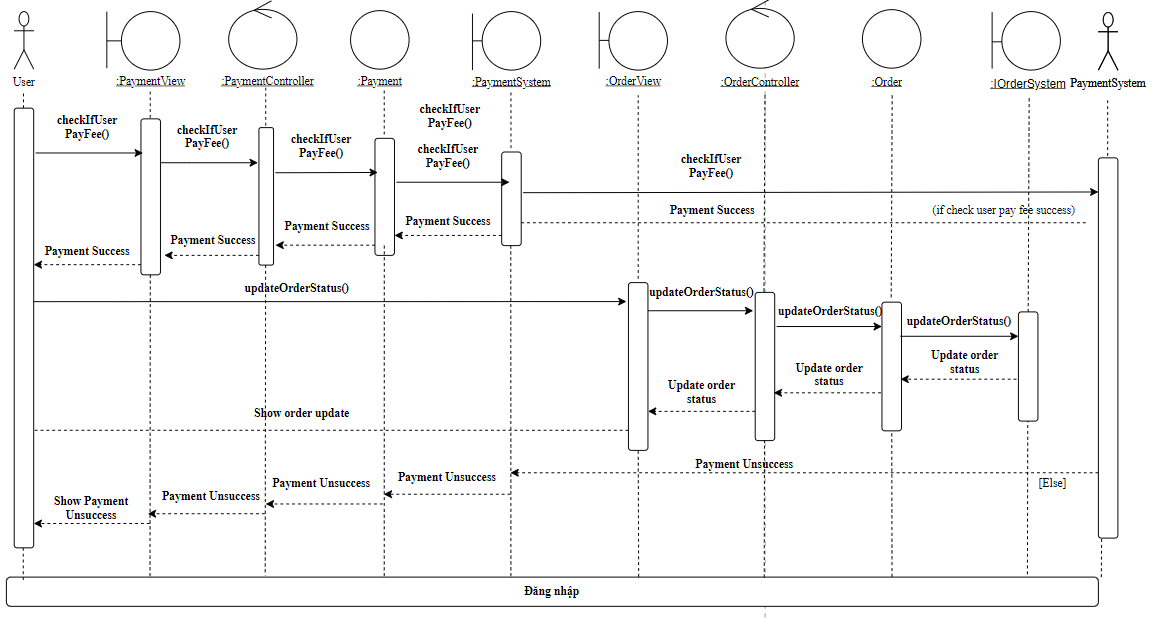
\includegraphics[width=\textwidth]{img2/2.1thanhtoantructiep.png}
    \caption{Biểu đồ tuần tự ca sử dụng Thanh toán trực tiếp}
\end{figure}

\subsubsection{Tra cứu phương tiện}
\begin{figure}[H]
    \centering
    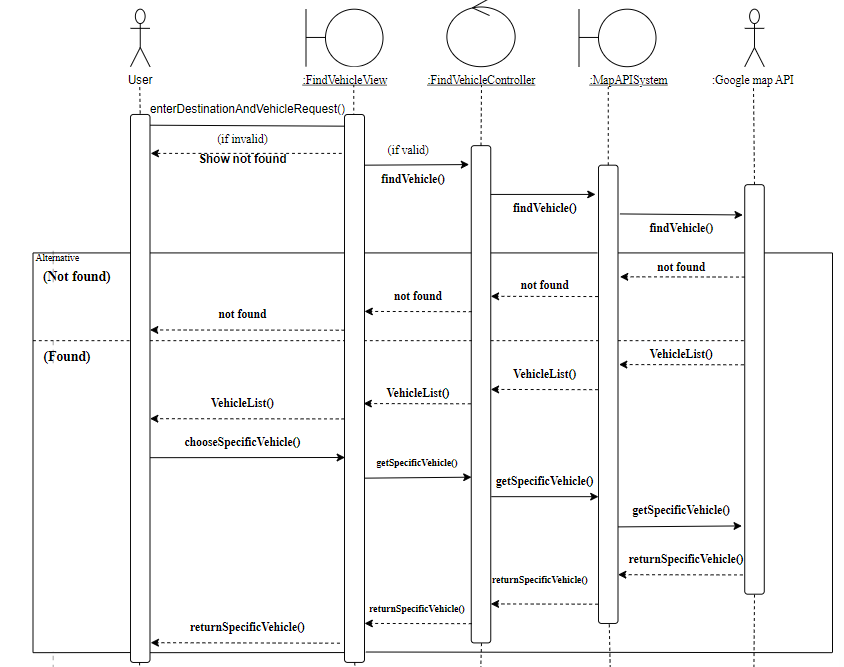
\includegraphics[width=\textwidth]{img2/2.1timphuongtien.png}
    \caption{Biểu đồ tuần tự ca sử dụng Tra cứu phương tiện}
\end{figure}

\subsubsection{Đăng ký tài khoản}
\begin{figure}[H]
    \centering
    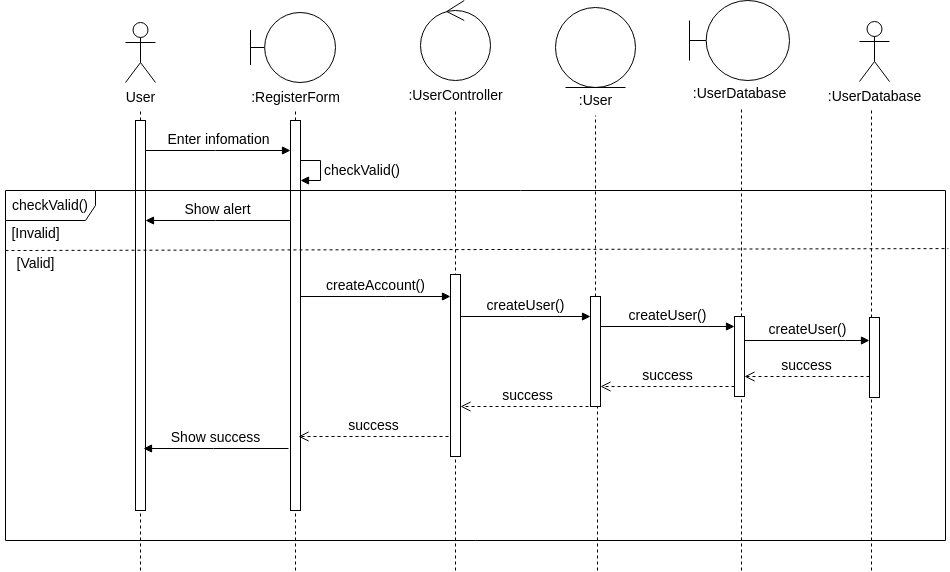
\includegraphics[width=\textwidth]{img2/Analysis-Đăng ký.drawio.png}
    \caption{Biểu đồ tuần tự ca sử dụng Đăng ký tài khoản}
\end{figure}

\subsubsection{Đăng nhập}
\begin{figure}[H]
    \centering
    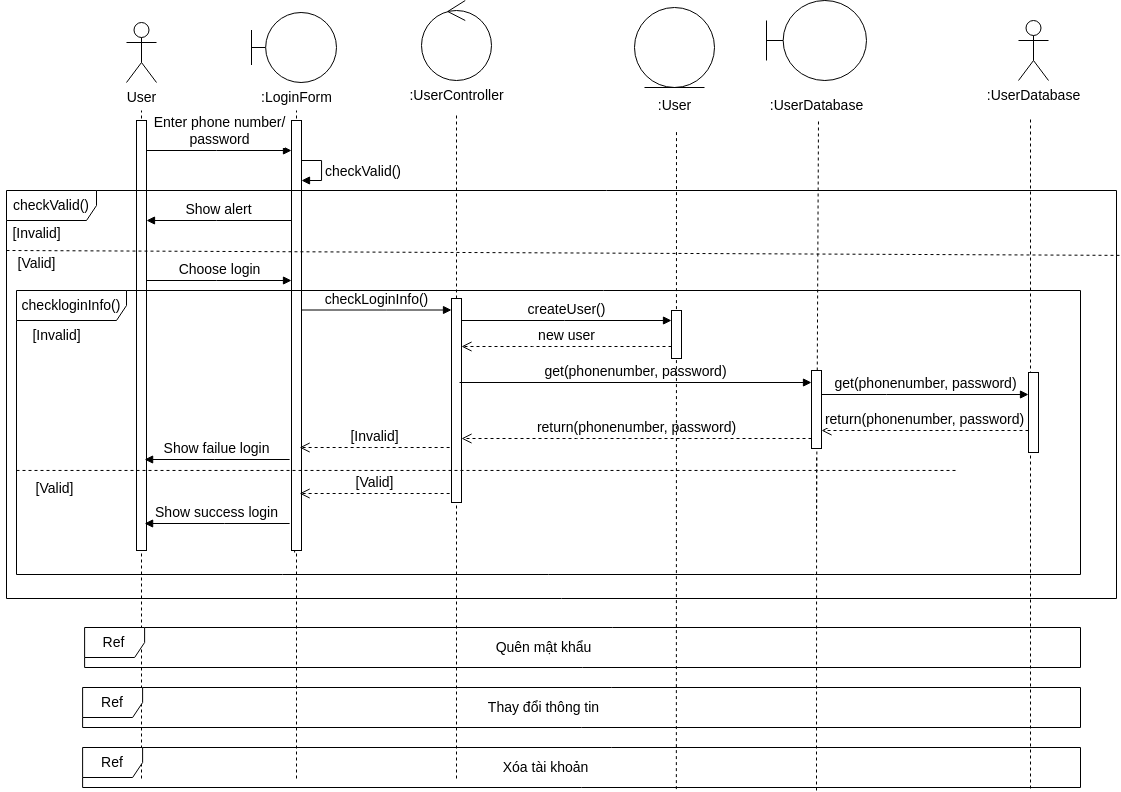
\includegraphics[width=\textwidth]{img2/Analysis-Đăng nhập.drawio.png}
    \caption{Biểu đồ tuần tự ca sử dụng Đăng nhập}
\end{figure}

\begin{figure}[H]
    \centering
    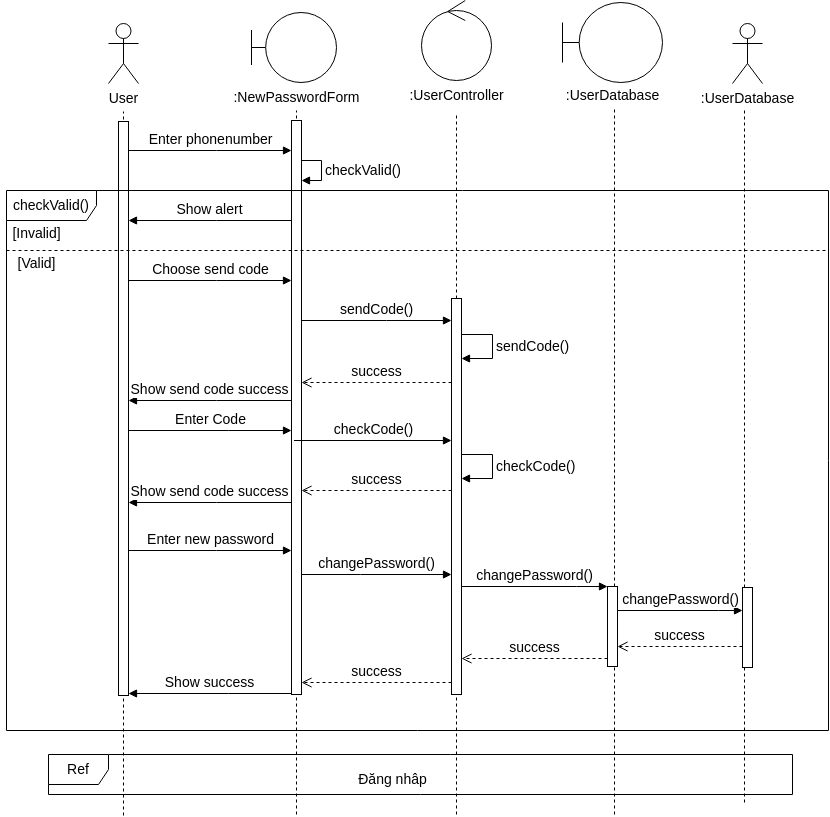
\includegraphics[width=\textwidth]{img2/Analysis-Đổi mật khẩu.drawio.png}
    \caption{Biểu đồ tuần tự ca sử dụng Quên mật khẩu}
\end{figure}

\begin{figure}[H]
    \centering
    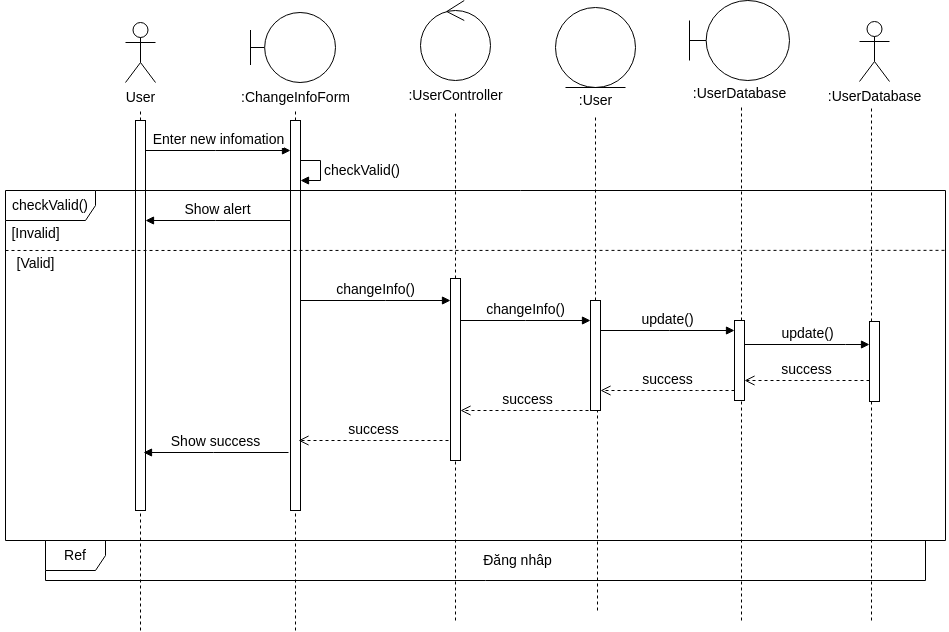
\includegraphics[width=\textwidth]{img2/Analysis-Thay đổi thông tin.drawio.png}
    \caption{Biểu đồ tuần tự ca sử dụng Thay đổi thông tin tài khoản}
\end{figure}

\begin{figure}[H]
    \centering
    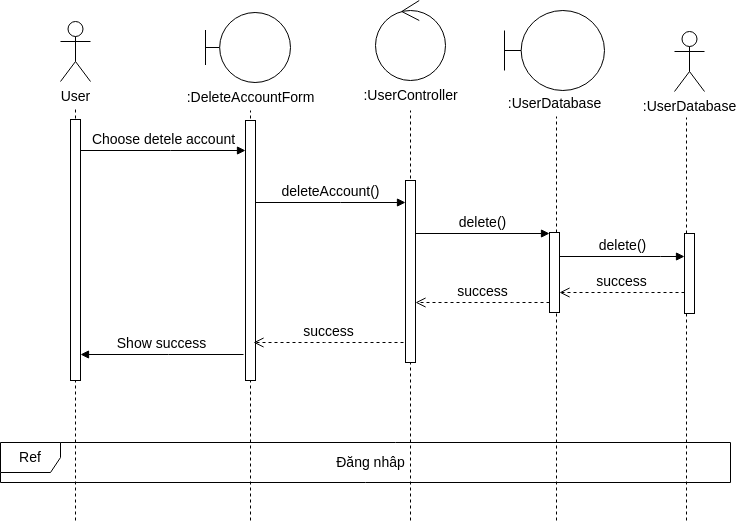
\includegraphics[width=0.9\textwidth]{img2/Analysis-Xóa tài khoản.drawio.png}
    \caption{Biểu đồ tuần tự ca sử dụng Xóa tài khoản}
\end{figure}

\subsubsection{Lựa chọn ngôn ngữ}
\begin{figure}[H]
    \centering
    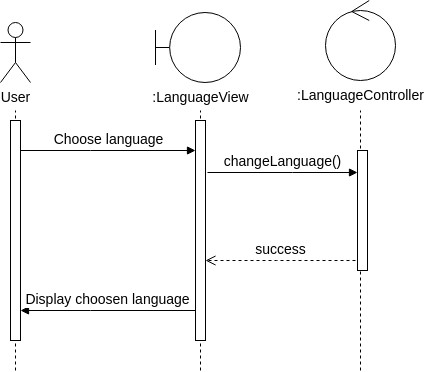
\includegraphics[width=0.7\textwidth]{img2/Analysis-Chọn ngôn ngữ.drawio.png}
    \caption{Biểu đồ tuần tự ca sử dụng Chọn ngôn ngữ}
\end{figure}

\subsection{Biểu đồ lớp pha phân tích}
\subsubsection{Đặt phòng khách sạn}
\begin{figure}[H]
    \centering
    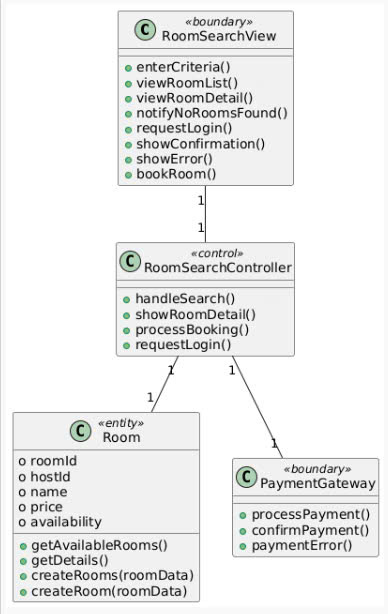
\includegraphics[width=0.8\textwidth]{img2.2/tim.jpg}
    \caption{Biểu đồ lớp cho ca sử dụng Đặt phòng khách sạn}
\end{figure}

\subsubsection{Theo dõi phòng đã đặt}
\begin{figure}[H]
    \centering
    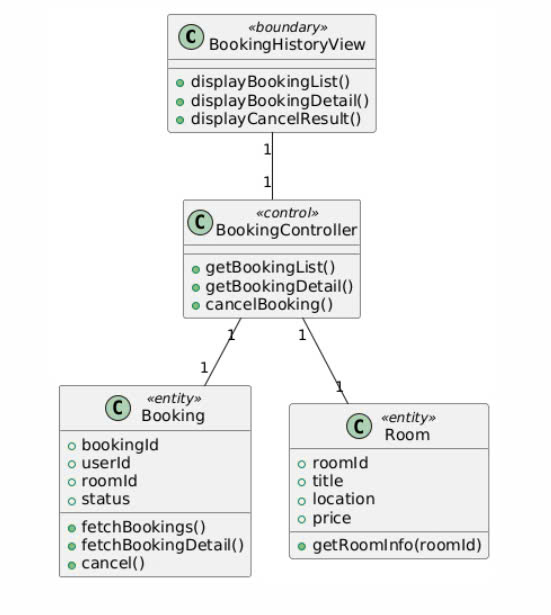
\includegraphics[width=\textwidth]{img2.2/dathue.jpg}
    \caption{Biểu đồ lớp ca sử dụng Theo dõi phòng đã đặt}
\end{figure}

\subsubsection{Đánh giá phòng đã thuê}
\begin{figure}[H]
    \centering
    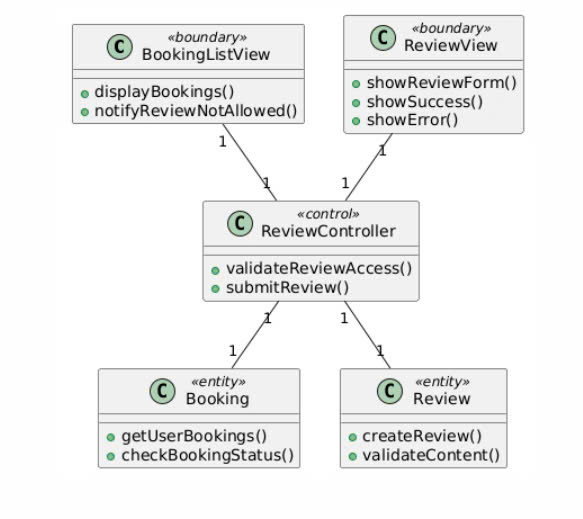
\includegraphics[width=\textwidth]{img2.2/nhaxet.jpg}
    \caption{Biểu đồ lớp ca sử dụng Đánh giá phòng đã thuê}
\end{figure}

\subsubsection{Liên hệ với chủ khách sạn}
\begin{figure}[H]
    \centering
    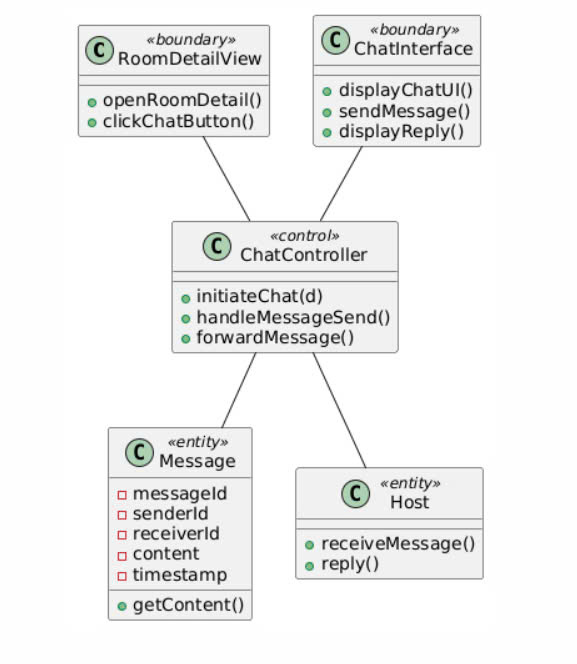
\includegraphics[width=\textwidth]{img2.2/ntin.jpg}
    \caption{Biểu đồ lớp ca sử dụng Liên hệ với chủ khách sạn}
\end{figure}

\subsubsection{Xem danh sách phòng yêu thích}
\begin{figure}[H]
    \centering
    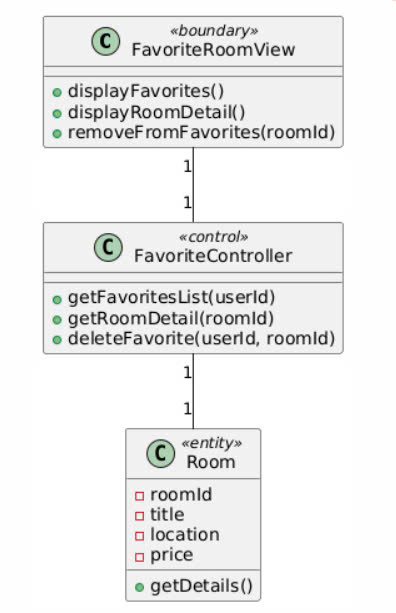
\includegraphics[width=0.4\textwidth]{img2.2/yeuthich.jpg}
    \caption{Biểu đồ lớp ca sử dụng Xem danh sách phòng yêu thích}
\end{figure}

\subsubsection{Cho thuê phòng}
\begin{figure}[H]
    \centering
    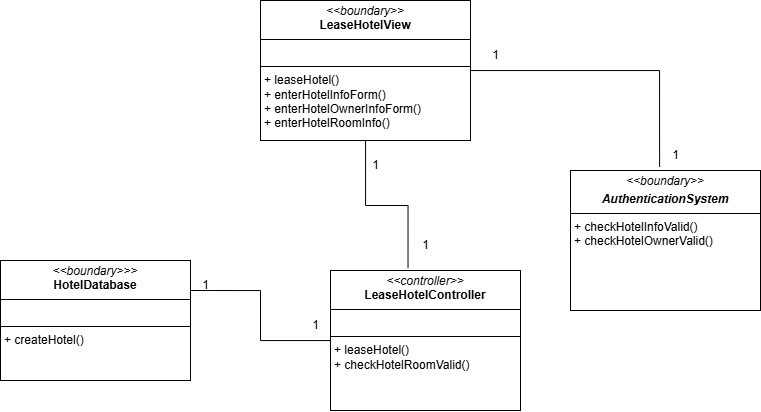
\includegraphics[width=0.9\textwidth]{img2.2/chothuephong.png}
    \caption{Biểu đồ lớp ca sử dụng Cho thuê phòng}
\end{figure}

\subsubsection{Chỉnh sửa thông tin phòng khách sạn}
\begin{figure}[H]
    \centering
    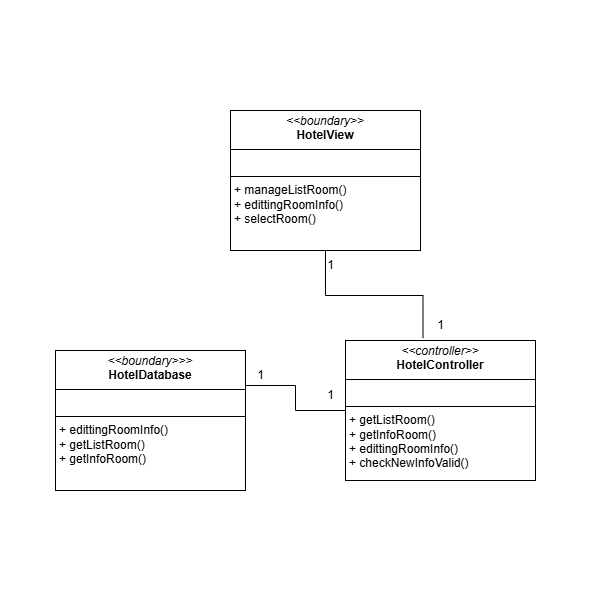
\includegraphics[width=0.6\textwidth]{img2.2/doithongtinphong.png}
    \caption{Biểu đồ lớp ca sử dụng Chỉnh sửa thông tin phòng khách sạn}
\end{figure}

\subsubsection{Tra cứu thông tin phòng cho thuê}
\begin{figure}[H]
    \centering
    \includegraphics[width=0.6\textwidth]{img2.2/tracuutrangthaiphong.png}
    \caption{Biểu đồ lớp ca sử dụng Tra cứu phòng cho thuê}
\end{figure}

\subsubsection{Xóa phòng khách sạn}
\begin{figure}[H]
    \centering
    \includegraphics[width=\textwidth]{img2.2/xoaphong.png}
    \caption{Biểu đồ lớp ca sử dụng Xóa phòng khách sạn}
\end{figure}

\subsubsection{Thanh toán}
\begin{figure}[H]
    \centering
    \includegraphics[width=\textwidth]{img2.2/2.2thanhtoan.png}
    \caption{Biểu đồ lớp ca sử dụng Thanh toán}
\end{figure}

\subsubsection{Tra cứu phương tiện}
\begin{figure}[H]
    \centering
    \includegraphics[width=\textwidth]{img2.2/2.2timphuongtien.png}
    \caption{Biểu đồ lớp ca sử dụng Tra cứu phương tiện}
\end{figure}

\subsubsection{Đăng ký tài khoản}
\begin{figure}[H]
    \centering
    \includegraphics[width=\textwidth]{img2.2/Analysis-Đăng ký.drawio.png}
    \caption{Biểu đồ lớp ca sử dụng Đăng ký tài khoản}
\end{figure}

\subsubsection{Đăng nhập}
\begin{figure}[H]
    \centering
    \includegraphics[width=\textwidth]{img2.2/Analysis-Đăng nhập.drawio.png}
    \caption{Biểu đồ lớp ca sử dụng Đăng nhập}
\end{figure}

\begin{figure}[H]
    \centering
    \includegraphics[width=\textwidth]{img2.2/Analysis-Quên mật khẩu.drawio.png}
    \caption{Biểu đồ lớp ca sử dụng Quên mật khẩu}
\end{figure}


\begin{figure}[H]
    \centering
    \includegraphics[width=\textwidth]{img2.2/Analysis-Thay đổi thông tin.drawio.png}
    \caption{Biểu đồ lớp ca sử dụng Thay đổi thông tin tài khoản}
\end{figure}

\begin{figure}[H]
    \centering
    \includegraphics[width=\textwidth]{img2.2/Analysis-Xóa tài khoản.drawio.png}
    \caption{Biểu đồ lớp ca sử dụng Xóa tài khoản}
\end{figure}

\subsubsection{Lựa chọn ngôn ngữ}
\begin{figure}[H]
    \centering
    \includegraphics[width=0.7\textwidth]{img2.2/Analysis-Thay đổi ngôn ngữ.drawio.png}
    \caption{Biểu đồ lớp ca sử dụng Chọn ngôn ngữ}
\end{figure}

\subsection{Ánh xạ từ lớp phân tích tới cơ chế phân tích}
\begin{longtable}{|p{6cm}|p{9cm}|}
\hline
\textbf{Analysis Class} & \textbf{Analysis Mechanism(s)} \\
\hline
RoomSearchView & None \\
\hline
RoomSearchController & Distribution \\
\hline
Room & Security, Persistency \\
\hline
PaymentGateway & Security, Error detection /handling /reporting \\
\hline
NotificationSystem & None \\
\hline
BookingHistoryView & None \\
\hline
BookingController & Distribution, Error detection /handling /reporting \\
\hline
Booking & Security, Persistency \\
\hline
BookingListView & None \\
\hline
ReviewView & None \\
\hline
ReviewController & Distribution \\
\hline
Review & Persistency, Security \\
\hline
RoomDetailView & None \\
\hline
ChatController & None \\
\hline
ChatInterface & None \\
\hline
Message & Persistency, Security \\
\hline
Host & Persistency, Security \\
\hline
FavoriteRoomView & None \\
\hline
FavoriteController & Distribution \\
\hline
Room & Persistency, Security \\
\hline
UserController & Distribution \\
\hline
LeaseHotelView & None \\
\hline
AuthenticationSystem & None \\
\hline
LeaseHotelController & Distribution \\
\hline
HotelDatabase & Persistency, Security \\
\hline
HotelView & None \\
\hline
HotelController & Distribution \\
\hline
SearchRentalHotelView & None \\
\hline
SearchRentalHotelController & Distribution \\
\hline
PaymentView & None \\
\hline
PaymentController & Distribution, Error detection /handling /reporting \\
\hline
Payment & Persistency, Security \\
\hline
PaymentSystem & Security, Error detection /handling /reporting \\
\hline
OrderView & None \\
\hline
OrderController & Distribution \\
\hline
Order & Persistency, Security \\
\hline
FindVehicleView & None \\
\hline
FindVehicleController & Distribution \\
\hline
LeaseHotelController & Distribution \\
\hline
MapAPISystem & None \\
\hline
RegisterForm & None \\
\hline
UserDatabase & Persistency, Security \\
\hline
User & Persistency, Security \\
\hline
LoginForm & None \\
\hline
NewPasswordForm & None \\
\hline
ChangeInfoForm & None \\
\hline
DeleteAccountForm & None \\
\hline
LanguageView & None \\
\hline
LanguageController & None \\
\hline
\end{longtable}
\chapter{Thiết kế hệ thống}
\section{Xác định các thành phần cần thiết kế}
\subsection{Subsystem Context}
\begin{figure}[H]
    \centering
    \includegraphics[width=\textwidth]{img3.1/userSubSystem(SubSystemContext).png} 
    \caption{User Subsystem Context}
\end{figure}

\begin{figure}[H]
    \centering
    \includegraphics[width=\textwidth]{img3.1/hotelSubSystem(SubSystemContext).png}
    \caption{Hotel Subsystem Context}
\end{figure}

\begin{figure}[H]
    \centering
    \includegraphics[width=\textwidth]{img3.1/paymentSy(SubSystemContext).png} 
    \caption{Payment Subsystem Context}
\end{figure}

\begin{figure}[H]
    \centering
    \includegraphics[width=0.9\textwidth]{img3.1/mapApi.png} 
    \caption{MapAPI System Context}
\end{figure}

\begin{figure}[H]
    \centering
    \includegraphics[width=0.9\textwidth]{img3.1/authentication.png} 
    \caption{Authentication System Context}
\end{figure}

\subsection{Analysis-to-Design-to-Implementation Mechanisms Map}
\begin{longtable}{|p{5cm}|p{4cm}|p{5cm}|}
\hline
\textbf{Cơ chế phân tích} & \textbf{Cơ chế thiết kế} & \textbf{Cơ chế cài đặt}\\
\hline
Persistency & OODBMS (new data) & ObjectStore \\
\hline
Persistency & RDBMS (data from
legacy database) & JDBC to Ingres \\
\hline
Distribution & Remote Method\newline
Invocation (RMI) & Java \\
\hline
Security & & Reverse Engineered\newline Secure.java and\newline UserContextRemoteObject components \\
\hline
Error detection/handling/reporting & & \\
\hline
\end{longtable}

\subsubsection{Cơ chế Persistency - ObjectStore OODBMS}
\textbf{Static View}
\begin{figure}[H]
    \centering
    \includegraphics[width=0.95\linewidth]{img3.1.2/design mechanism-Persistency.drawio.png}
\end{figure}
\begin{itemize}
    \item Trong JDBC, một máy khách sẽ làm việc với \textbf{DBClass} để đọc và ghi dữ liệu. DBClass chịu trách nhiệm truy cập cơ sở dữ liệu JDBC bằng lớp \textbf{DriverManager}. Khi một Kết nối cơ sở dữ liệu được mở, DBClass sau đó có thể tạo các câu lệnh SQL sẽ được gửi đến RDBMS cơ bản và được thực thi bằng lớp \textbf{Statement}. Lớp Statement là lớp "nói chuyện" với cơ sở dữ liệu. Kết quả của truy vấn SQL được trả về trong một đối tượng \textbf{ResultSet}.
    \item Lớp \textbf{DBClass} chịu trách nhiệm tạo ra instnce của một lớp. Nó có cơ chế ánh xạ OO-to-RDBMS và có hành vi để giao tiếp với RDBMS. DBClass làm phẳng đối tượng, ghi nó vào RDBMS và đọc dữ liệu đối tượng từ RDBMS và xây dựng đối tượng đó. Mỗi lớp persistency sẽ có một DBClass tương ứng.
    \item \textbf{PersistentClassList} được sử dụng để trả về một tập hợp các đối tượng persistency là kết quả của truy vấn cơ sở dữ liệu.
\end{itemize}

\textbf{Dynamic View}
\begin{figure}[H]
    \centering
    \includegraphics[width=0.75\linewidth]{img3.1.2/design mechanism-Initialize.drawio.png}
    \caption{Initialize}
\end{figure}
Bước khởi tạo phải có trước khi các lớp khác có thể kết nối. Để khởi tạo kết nối tới cơ sở dữ liệu, DBClass phải gọi hàm getConnection(). Và phương thức getConnection() sẽ tạo một kết nối với URL đã nhập sau đó trả về kết nối này.

\begin{figure}[H]
    \centering
    \includegraphics[width=\linewidth]{img3.1.2/design mechanism-Create.drawio.png}
    \caption{Create}
\end{figure}
Để tạo một lớp mới, DBClass tạo một thể hiện mới của PersistentClass với các giá trị mặc định. Sau đó, DBClass tạo một Statement mới bằng cách sử dụng phương thức createStatement() của lớp Connection. Statement được thực thi và dữ liệu được chèn vào cơ sở dữ liệu.

\begin{figure}[H]
    \centering
    \includegraphics[width=\linewidth]{img3.1.2/design mechanism-Read.drawio.png}
    \caption{Read}
\end{figure}
Để đọc dữ liệu, DBClass tạo một Statement mới bằng cách sử dụng createStatement() của lớp Connection. Statement được thực thi và dữ liệu được trả về trong một đối tượng ResultSet. Sau đó, DBClass tạo một thể hiện mới của PersistentClass và điền vào đó dữ liệu đã truy xuất. Dữ liệu được trả về trong một đối tượng collection, một thể hiện của lớp PersistentClassList.

\begin{figure}[H]
    \centering
    \includegraphics[width=0.9\linewidth]{img3.1.2/design mechanism-Update.drawio.png}
    \caption{Update}
\end{figure}
Để cập nhật dữ liệu, DBClass lấy dữ liệu từ đối tượng PersistentClass đã cho và tạo một Statement mới bằng cách sử dụng phương thức createStatement() của lớp Connection. Sau khi Statement được xây dựng, bản cập nhật được thực thi và cơ sở dữ liệu được cập nhật với dữ liệu mới.

\begin{figure}[H]
    \centering
    \includegraphics[width=0.9\linewidth]{img3.1.2/design mechanism-Delete.drawio.png}
    \caption{Delete}
\end{figure}
Để xóa dữ liệu, DBClass tạo một Statement mới bằng cách sử dụng phương thức createStatement() của lớp Connection. Statement được thực thi và dữ liệu được xóa khỏi cơ sở dữ liệu.

\subsubsection{Cơ chế Distribution}
\textbf{Static View}
\begin{figure}[H]
    \centering
    \includegraphics[width=\linewidth]{img3.1.2/design mechanism-Distribution.drawio.png}
\end{figure}

\begin{itemize}
    \item Cả client và server đều là hệ thống hướng đối tượng. Tương tác giữa server và client được đóng gói trong một hoặc nhiều đối tượng có thể truy cập từ xa. Các đối tượng này được khởi tạo trên server, nhưng client xử lý đối tượng như thể chúng là các khởi tạo cục bộ.
    \item Các stub và skeleton là các adapter, đầu tiên giúp client thích ứng với Internet và sau đó là Internet thích ứng với đối tượng của server.
    \item Bất kỳ đối tượng có thể tuần tự hóa nào đều có thể được truyền đến máy chủ bằng cách sử dụng tham số đầu vào nếu là phương thức của giao diện IRemoteObject.
    \item Bất kỳ phương thức nào mà client chạy trên đối tượng từ xa đều thực sự chạy trên server.
    \item Bất kỳ phương thức nào của đối tượng không phải UnicastRemoteObject có thể tuần tự hóa được đặt cho client đều chạy trên client.
    \item Lớp sercer phải chạy để RMIRegistry có thể tải các stub ban đầu để chuẩn bị truyền chúng tới client.
\end{itemize}

\textbf{Dynamic View}
\begin{figure}[H]
    \centering
    \includegraphics[width=0.9\linewidth]{img3.1.2/design mechanism-Page-8.drawio.png}
\end{figure}
\subsubsection{Cơ chế Security}
\textbf{Static View}
\begin{figure}[H]
    \centering
    \includegraphics[width=0.8\linewidth]{img3.1.2/design mechanism-Sercurity.drawio.png}
\end{figure}
\begin{itemize}
    \item ISecureData: cơ chế phân tích: security
    \item SecurityAccess: cơ chế phân tích: security
    \item UserSecurityContext: cơ chế phân tích: security
    \item UniqueId: cơ chế phân tích: security
    \item IUserSubsystem: cơ chế phân tích: security
    \item ISecureUser: cơ chế phân tích: security
    \item UserController: cơ chế phân tích: security
\end{itemize}

\textbf{Dynamic View}
\begin{figure}[H]
    \centering
    \includegraphics[width=1.1\linewidth]{img3.1.2/design mechanism-seq secure.drawio.png}
\end{figure}

\subsection{Analysis-Class-to-Design-Element Map}
\begin{longtable}{|p{6cm}|p{9cm}|}
\hline
\textbf{Analysis Class} & \textbf{Design Elements} \\
\hline
RoomSearchView & RoomSearchForm \\
\hline
RoomSearchController & RoomService \\
\hline
Room & Room \\
\hline
PaymentGateway & PaymentService \\
\hline
NotificationSystem & NotificationService\\
\hline
BookingHistoryView & BookingHistoryView \\
\hline
BookingController & BookingController, BookingRepository \\
\hline
Booking & Booking \\
\hline
BookingListView & BookingListView \\
\hline
ReviewView & ReviewView \\
\hline
ReviewController & ReviewController, ReviewRepository \\
\hline
Review & Review \\
\hline
RoomDetailView & RoomDetailView \\
\hline
ChatController & ChatController, ChatRepository \\
\hline
ChatInterface & ChatInterface \\
\hline
Message & Message,  MessageService \\
\hline
Host & Host \\
\hline
FavoriteRoomView & FavoriteRoomView \\
\hline
FavoriteController & FavoriteController, FavorieRepository \\
\hline
Room & Room \\
\hline
UserController & UserController \\
\hline
LeaseHotelView & LeaseHotelView \\
\hline
AuthenticationSystem & AuthenticationSystem \\
\hline
LeaseHotelController & LeaseHotelController \\
\hline
HotelDatabase & HotelDatabase \\
\hline
HotelView & HotelView \\
\hline
HotelController & HotelController, IHotelSubSystem \\
\hline
SearchRentalHotelView & SearchRentalHotelView \\
\hline
SearchRentalHotelController & SearchRentalHotelController \\
\hline
PaymentView & PaymentView \\
\hline
PaymentController & PaymentController \\
\hline
Payment & Payment \\
\hline
PaymentSystem & IPaymentSystem \\
\hline
OrderView & OrderView \\
\hline
OrderController & OrderController, IOrderSystem \\
\hline
Order & Order \\
\hline
FindVehicleView & FindVehicleView \\
\hline
FindVehicleController & FindVehicleController \\
\hline
LeaseHotelController & LeaseHotelController \\
\hline
AuthenticationSystem & IAuthentifacationSubSystem\\
\hline
MapAPISystem & ImapAPI \\
\hline
RegisterForm & RegisterForm \\
\hline
UserDatabase & UserDatabase \\
\hline
User & User, IUserSubsystem \\
\hline
LoginForm & LoginForm \\
\hline
NewPasswordForm & NewPasswordForm \\
\hline
ChangeInfoForm & ChangeInfoForm \\
\hline
DeleteAccountForm &DeleteAccountForm \\
\hline
LanguageView & LanguageView \\
\hline
LanguageController & LanguageController \\
\hline
\end{longtable}

\subsection{Design-Element-to-Owning-Package Map}
\begin{longtable}{|p{6cm}|p{9cm}|}
\hline
\textbf{Design Elements
Owni} & \textbf{Owning package} \\
\hline
RoomSearchForm & GUI\_Management \\
\hline
RoomService & Subsystem.HotelSubsystem \\
\hline
Room & Database.Hotelinfo \\
\hline
PaymentService & Subsystem.PaymentSystem \\
\hline
NotificationService & Subsystem \\
\hline
BookingHistoryView & GUI\_Management \\
\hline
BookingController & Subsystem.BookingSubsystem \\
\hline
BookingRepository & Subsystem.BookingSubsystem \\
\hline
Booking & Database.Bookingdata\\
\hline
BookingListView & GUI\_Management \\
\hline
ReviewView & GUI\_Management \\
\hline
ReviewController & Database.ReviewSubsystem \\
\hline
ReviewRepository & Subsystem.ReviewSubsystem \\
\hline
Review & Database.Reviewdata \\
\hline
RoomDetailView & GUI\_Management \\
\hline
ChatController & Subsystem.ChatSubsystem \\
\hline
ChatRepository & Subsystem.ChatSubsystem \\
\hline
ChatInterface &  Subsystem.ChatSubsystem\\
\hline
Message & Database.Bookingdata\\
\hline
MessageService & Subsystem.ChatSubsystem \\
\hline
Host & Database.Userdata \\
\hline
FavoriteRoomView & GUI\_Management \\
\hline
FavoriteController & Subsystem.BookingSubsystem \\ 
\hline
FavorieRepository & Subsystem.BookingSubsystem \\
\hline
Room & Database.hoteldata \\
\hline
UserController & Subsystem.UserSubsystem \\
\hline
LeaseHotelView & GUI\_Management \\
\hline
AuthenticationSystem & Subsystem \\
\hline
LeaseHotelController & Subsystem.BookingSubsystem \\
\hline
HotelDatabase & Database.Hoteldata \\
\hline
HotelView & GUI\_Management \\
\hline
HotelController & Subsystem.HotelSubsystem \\
\hline
IHotelSubSystem & Subsystem.HotelSubsystem \\
\hline
SearchRentalHotelView & GUI\_Management \\
\hline
SearchRentalHotelController & Subsystem.BookingSubsystem \\
\hline
PaymentView & GUI\_Management \\
\hline
PaymentController & Subsystem.PaymentSystem \\
\hline
Payment & Database.Bookingdata \\
\hline
PaymentSystem & Subsystem.PaymentSystem \\
\hline
OrderView & GUI\_Management \\
\hline
OrderController & Subsystem.BookingSubsystem \\
\hline
IOrderSystem & Subsystem.BookingSubsystem \\
\hline
Order & Database.Bookingdata \\
\hline
FindVehicleView & GUI\_Management \\
\hline
FindVehicleController & Subsystem.BookingSubsystem \\
\hline
LeaseHotelController & Subsystem.BookingSubsystem \\
\hline
AuthenticationSystem & Subsystem\\
\hline
MapAPISystem & GUI\_Management \\
\hline
RegisterForm & GUI\_Management \\
\hline
UserDatabase & Database.Userdata \\
\hline
User & Database.Userdata\\ 
\hline
IUserSubsystem & Subsystem.UserSubsystem \\
\hline
LoginForm & GUI\_Management \\
\hline
NewPasswordForm & GUI\_Management \\
\hline
ChangeInfoForm & GUI\_Management \\
\hline
DeleteAccountForm & GUI\_Management \\
\hline
LanguageView & GUI\_Management \\
\hline
LanguageController & Subsystem \\
\hline
\end{longtable}

\subsection{Packages and Their Dependency}
\begin{figure}[H]
    \centering
    \includegraphics[width=\textwidth]{img3.1.5/Blank 2 Grids Collage_0.jpg} 
\end{figure}

\section{Mô tả kiến trúc thực thi}
\begin{figure}[H]
    \centering
    \includegraphics[width=\linewidth]{img3.2/1.jpg}
\end{figure}

\section{Thiết kế Use Case }

\subsection{Thiết kế biểu đồ tuần tự}
\subsubsection{Đặt phòng khách sạn}
\begin{figure}[H]
    \centering
    \includegraphics[width=\textwidth]{img3.4/timphong3.jpg} 
    \caption{Biểu đồ tuần tự Đặt phòng khách sạn}
\end{figure}

\subsubsection{Theo dõi phòng đã đặt}
\begin{figure}[H]
    \centering
    \includegraphics[width=\textwidth]{img3.4/xemphongthue3.jpg} 
    \caption{Biểu đồ tuần tự Theo dõi phòng đã đặt}
\end{figure}

\subsubsection{Đánh giá phòng đã thuê}
\begin{figure}[H]
    \centering
    \includegraphics[width=\textwidth]{img3.4/dgia3.jpg} 
    \caption{Biểu đồ tuần tự Đánh giá phòng đã thuê}
\end{figure}

\subsubsection{Liên hệ với chủ khách sạn}
\begin{figure}[H]
    \centering
    \includegraphics[width=\textwidth]{img3.4/chat3.jpg} 
    \caption{Biểu đồ tuần tự Liên hệ với chủ khách sạn}
\end{figure}

\subsubsection{Xem danh sách phòng yêu thích}
\begin{figure}[H]
    \centering
    \includegraphics[width=\textwidth]{img3.4/xemphongyeu3.jpg} 
    \caption{Biểu đồ tuần tự Xem danh sách phòng yêu thích}
\end{figure}

\subsubsection{Cho thuê phòng}
\begin{figure}[H]
    \centering
    \includegraphics[width=\textwidth]{img3.4/chothuephong.png} 
    \caption{Biểu đồ tuần tự Cho thuê phòng}
\end{figure}

\subsubsection{Sửa thông tin phòng}
\begin{figure}[H]
    \centering
    \includegraphics[width=0.75\textwidth]{img3.4/doitrangthaiphong.jpg} 
    \caption{Biểu đồ tuần tự Sửa thông tin phòng}
\end{figure}

\subsubsection{Tra cứu thông tin phòng đang cho thuê}
\begin{figure}[H]
    \centering
    \includegraphics[width=\textwidth]{img3.4/tracuutheotrangthai.jpg} 
    \caption{Biểu đồ tuần tự Tra cứu phòng theo trạng thái}
\end{figure}

\begin{figure}[H]
    \centering
    \includegraphics[width=\textwidth]{img3.4/tracuutheodoanhthu.jpg} 
    \caption{Biểu đồ tuần tự Tra cứu doanh thu phòng}
\end{figure}

\subsubsection{Xóa phòng khách sạn}
\begin{figure}[H]
    \centering
    \includegraphics[width=0.95\textwidth]{img3.4/xoaphong.jpg} 
    \caption{Biểu đồ tuần tự Xóa phòng khách sạn}
\end{figure}

\subsubsection{Thanh toán}
\begin{figure}[H]
    \centering
    \includegraphics[width=\textwidth]{img3.4/3.4.1thanhtoanbangtk.png} 
    \caption{Biểu đồ tuần tự Thanh toán trực tuyến}
\end{figure}

\begin{figure}[H]
    \centering
    \includegraphics[width=\textwidth]{img3.4/3.4.1thanhtoantructiep.png} 
    \caption{Biểu đồ tuần tự Thanh toán trực tiếp}
\end{figure}

\subsubsection{Tra cứu phương tiện}
\begin{figure}[H]
    \centering
    \includegraphics[width=\textwidth]{img3.4/3.4.1 timphuongtien.png} 
    \caption{Biểu đồ tuần tự Tra cứu phương tiện}
\end{figure}

\subsubsection{Đăng ký tài khoản}
\begin{figure}[H]
    \centering
    \includegraphics[width=\textwidth]{img3.4/Design_diagram-Đăng ký.drawio.png} 
    \caption{Biểu đồ tuần tự Đăng ký tài khoản}
\end{figure}

\subsubsection{Đăng nhập}
\begin{figure}[H]
    \centering
    \includegraphics[width=\textwidth]{img3.4/Design_diagram-Đăng nhập.drawio.png} 
    \caption{Biểu đồ tuần tự Đăng nhập}
\end{figure}

\begin{figure}[H]
    \centering
    \includegraphics[width=\textwidth]{img3.4/Design_diagram-Quên mật khẩu.drawio.png} 
    \caption{Biểu đồ tuần tự Quên mật khẩu}
\end{figure}

\begin{figure}[H]
    \centering
    \includegraphics[width=\textwidth]{img3.4/Design_diagram-Thay đổi thông tin.drawio.png} 
    \caption{Biểu đồ tuần tự Thay đổi thông tin tài khoản}
\end{figure}

\begin{figure}[H]
    \centering
    \includegraphics[width=\textwidth]{img3.4/Design_diagram-Xóa tài khoản.drawio.png} 
    \caption{Biểu đồ tuần tự Xóa tài khoản}
\end{figure}

\subsubsection{Lựa chọn ngôn ngữ}
\begin{figure}[H]
    \centering
    \includegraphics[width=\textwidth]{img3.4/Design_diagram-Chọn ngôn ngữ.drawio.png} 
    \caption{Biểu đồ tuần tự Lựa chọn ngôn ngữ}
\end{figure}

\subsection{Thiết kế biểu đồ lớp}
\subsubsection{Đặt phòng khách sạn}
\begin{figure}[H]
    \centering
    \includegraphics[width=\textwidth]{img3.4.2/thuephong4.jpg} 
    \caption{Biểu đồ lớp Đặt phòng khách sạn}
\end{figure}

\subsubsection{Theo dõi phòng đã đặt}
\begin{figure}[H]
    \centering
    \includegraphics[width=\textwidth]{img3.4.2/xemphongthue4.jpg} 
    \caption{Biểu đồ lớp Theo dõi phòng đã đặt}
\end{figure}


\subsubsection{Đánh giá phòng đã thuê}
\begin{figure}[H]
    \centering
    \includegraphics[width=\textwidth]{img3.4.2/dgia4.jpg} 
    \caption{Biểu đồ lớp Đánh giá phòng đã thuê}
\end{figure}


\subsubsection{Liên hệ với chủ khách sạn}
\begin{figure}[H]
    \centering
    \includegraphics[width=\textwidth]{img3.4.2/chat4.jpg} 
    \caption{Biểu đồ lớp Liên hệ với chủ khách sạn}
\end{figure}

\subsubsection{Xem danh sách phòng yêu thích}
\begin{figure}[H]
    \centering
    \includegraphics[width=\textwidth]{img3.4.2/xemphongyeu4.jpg} 
    \caption{Biểu đồ lớp Xem danh sách phòng yêu thích}
\end{figure}

\subsubsection{Cho thuê phòng}
\begin{figure}[H]
    \centering
    \includegraphics[width=0.7\textwidth]{img3.4.2/chothuephong.png} 
    \caption{Biểu đồ lớp Cho thuê phòng}
\end{figure}

\subsubsection{Sửa thông tin phòng}
\begin{figure}[H]
    \centering
    \includegraphics[width=0.55\textwidth]{img3.4.2/doithongtinphong.jpg} 
    \caption{Biểu đồ lớp Sửa thông tin phòng}
\end{figure}

\subsubsection{Tra cứu thông tin phòng đang cho thuê}
\begin{figure}[H]
    \centering
    \includegraphics[width=\textwidth]{img3.4.2/tracuuphong.jpg} 
    \caption{Biểu đồ lớp Tra cứu thông tin phòng đang cho thuê}
\end{figure}

\subsubsection{Xóa phòng khách sạn}
\begin{figure}[H]
    \centering
    \includegraphics[width=0.8\textwidth]{img3.4.2/xoaphong.jpg} 
    \caption{Biểu đồ lớp Xóa phòng khách sạn}
\end{figure}

\subsubsection{Thanh toán}
\begin{figure}[H]
    \centering
    \includegraphics[width=\textwidth]{img3.4.2/3.4.2thanhtoanbangtk.png} 
    \caption{Biểu đồ lớp Thanh toán trực tuyến}
\end{figure}

\begin{figure}[H]
    \centering
    \includegraphics[width=\textwidth]{img3.4.2/3.4.2thanhtoantructiep.png} 
    \caption{Biểu đồ lớp Thanh toán trực tiếp}
\end{figure}

\subsubsection{Tra cứu phương tiện}
\begin{figure}[H]
    \centering
    \includegraphics[width=\textwidth]{img3.4.2/3.4.2timphuongtien.png} 
    \caption{Biểu đồ lớp Tra cứu phương tiện}
\end{figure}

\subsubsection{Đăng ký tài khoản}
\begin{figure}[H]
    \centering
    \includegraphics[width=\textwidth]{img3.4.2/Design_diagram-Lớp đăng ký.drawio.png} 
    \caption{Biểu đồ lớp Đăng ký tài khoản}
\end{figure}

\subsubsection{Đăng nhập}
\begin{figure}[H]
    \centering
    \includegraphics[width=0.9\textwidth]{img3.4.2/Design_diagram-Lớp đăng nhập.drawio.png} 
    \caption{Biểu đồ lớp Đăng nhập}
\end{figure}

\begin{figure}[H]
    \centering
    \includegraphics[width=0.9\textwidth]{img3.4.2/Design_diagram-Lớp quên mật khẩu.drawio.png} 
    \caption{Biểu đồ lớp Quên mật khẩu}
\end{figure}

\begin{figure}[H]
    \centering
    \includegraphics[width=\textwidth]{img3.4.2/Design_diagram-Lớp thay đổi thông tin.drawio.png} 
    \caption{Biểu đồ lớp Thay đổi thông tin tài khoản}
\end{figure}

\begin{figure}[H]
    \centering
    \includegraphics[width=\textwidth]{img3.4.2/Design_diagram-Lớp xóa tài khoản.drawio.png} 
    \caption{Biểu đồ lớp Xóa tài khoản}
\end{figure}

\subsubsection{Lựa chọn ngôn ngữ}
\begin{figure}[H]
    \centering
    \includegraphics[width=\textwidth]{img3.4.2/Design_diagram-Lớp chọn ngôn ngữ.drawio.png} 
    \caption{Biểu đồ lớp Lựa chọn ngôn ngữ}
\end{figure}

\section{Thiết kế Hệ thống con}
\subsection{User Subsystem}
\begin{figure}[H]
    \centering
    \includegraphics[width=\textwidth]{img3.5/user/cauTruc(UserSst).png} 
    \caption{Biểu đồ cấu trúc UserSubsystem}
\end{figure}

\begin{figure}[H]
    \centering
    \includegraphics[width=\textwidth]{img3.5/user/quanHe(UserSst).png} 
    \caption{Biểu đồ quan hệ UserSubsystem}
\end{figure}
\textbf{Interface IUserSubsystem}
    \begin{enumerate}
        \item Hàm changePassword()
        \begin{figure}[H]
        \centering
        \includegraphics[width=0.7\linewidth]{img3.5/user/changePassword.png}
        \end{figure}
        \item Hàm checkLogin()
        \begin{figure}[H]
        \centering
        \includegraphics[width=0.8\linewidth]{img3.5/user/checkLogin.png} 
        \end{figure}
        \item Hàm createAccount()
        \begin{figure}[H]
        \centering
        \includegraphics[width=0.75\linewidth]{img3.5/user/createAccount.png} 
        \end{figure}
        \item Hàm deleteUser()
        \begin{figure}[H]
        \centering
        \includegraphics[width=0.7\linewidth]{img3.5/user/deleteUser.png} 
        \end{figure}
        \item Hàm updateUser()
        \begin{figure}[H]
        \centering
        \includegraphics[width=0.875\linewidth]{img3.5/user/updateUser.png} 
        \end{figure}
        \item Hàm checkDuplicate()
        \begin{figure}[H]
        \centering
        \includegraphics[width=0.7\linewidth]{img3.5/user/checkDuplicate.png}
        \end{figure}
        \item Hàm verifyPaymentCode()
        \begin{figure}[H]
        \centering
        \includegraphics[width=0.7\linewidth]{img3.5/user/verifyPaymentCode.png}
        \end{figure}
    \end{enumerate}

\subsection{Hotel Subsystem}
\begin{figure}[H]
    \centering
    \includegraphics[width=\textwidth]{img3.5/hotel/hotelsubsystem1.drawio (1).png} 
    \caption{Biểu đồ cấu trúc HotelSubSystem}
\end{figure}

\begin{figure}[H]
    \centering
    \includegraphics[width=\textwidth]{img3.5/hotel/newHotelSub.png} 
    \caption{Biểu đồ quan hệ HotelSubSystem}
\end{figure}

\textbf{Interface IHotelSubsystem}
    \begin{enumerate}
        \item Hàm leaseHotel()
        \begin{figure}[H]
        \centering
        \includegraphics[width=0.8\linewidth]{img3.5/hotel/leaseHotel.jpg} 
        \end{figure}
        \item Hàm deleteRoom()
        \begin{figure}[H]
        \centering
        \includegraphics[width=0.8\linewidth]{img3.5/hotel/deleteRoom.png} 
        \end{figure}
        \item Hàm edittingRoomInfo()
        \begin{figure}[H]
        \centering
        \includegraphics[width=0.8\linewidth]{img3.5/hotel/edittingRoomInfo.png} 
        \end{figure}
        \item Hàm getRoomsByRenenue()
        \begin{figure}[H]
        \centering
        \includegraphics[width=0.8\linewidth]{img3.5/hotel/getRoomsByRenenue.png} 
        \end{figure}
        \item Hàm getRoomsByStatus()
        \begin{figure}[H]
        \centering
        \includegraphics[width=0.85\linewidth]{img3.5/hotel/getRoomByStatus.png} 
        \end{figure}
        \item Hàm bookingRoom()
        \begin{figure}[H]
        \centering
        \includegraphics[width=0.9\linewidth]{img3.5/hotel/newbookingRoom.png} 
        \end{figure}
        \item Hàm exchangeWithOwner()
        \begin{figure}[H]
        \centering
        \includegraphics[width=0.9\linewidth]{img3.5/hotel/exchangeWithOwner.png} 
        \end{figure}
        \item Hàm reviewRoom()
        \begin{figure}[H]
        \centering
        \includegraphics[width=0.95\linewidth]{img3.5/hotel/reviewRoom.png} 
        \end{figure}
        \item Hàm getBookedRoom()
        \begin{figure}[H]
        \centering
        \includegraphics[width=\linewidth]{img3.5/hotel/getBookedRoom.png} 
        \end{figure}
    \end{enumerate}

\section{Thiết kế lớp}
\begin{figure}[H]
    \centering
    \includegraphics[width=\linewidth]{img3.6/1.png}
\end{figure}
\begin{figure}[H]
    \centering
    \includegraphics[width=\linewidth]{img3.6/2.png}
\end{figure}
\begin{figure}[H]
    \centering
    \includegraphics[width=\linewidth]{img3.6/3.png}
\end{figure}
\begin{figure}[H]
    \centering
    \includegraphics[width=\linewidth]{img3.6/4.png}
\end{figure}
\begin{figure}[H]
    \centering
    \includegraphics[width=\linewidth]{img3.6/5.png}
\end{figure}
\begin{figure}[H]
    \centering
    \includegraphics[width=\linewidth]{img3.6/6.png}
\end{figure}
\begin{figure}[H]
    \centering
    \includegraphics[width=\linewidth]{img3.6/7.png}
\end{figure}
\begin{figure}[H]
    \centering
    \includegraphics[width=\linewidth]{img3.6/8.png}
\end{figure}
\begin{figure}[H]
    \centering
    \includegraphics[width=\linewidth]{img3.6/9.png}
\end{figure}
\begin{figure}[H]
    \centering
    \includegraphics[width=\linewidth]{img3.6/10.png}
\end{figure}
\begin{figure}[H]
    \centering
    \includegraphics[width=0.8\linewidth]{img3.6/11.png}
\end{figure}
\begin{figure}[H]
    \centering
    \includegraphics[width=0.8\linewidth]{img3.6/12.png}
\end{figure}
\begin{figure}[H]
    \centering
    \includegraphics[width=\linewidth]{img3.6/13.png}
\end{figure}
\begin{figure}[H]
    \centering
    \includegraphics[width=\linewidth]{img3.6/14.png}
\end{figure}

\section{Thiết kế Cơ sở dữ liệu}
\begin{figure}[H]
    \centering
    \includegraphics[width=\linewidth]{img3.7/3.7.png}
\end{figure}

\textbf{Bảng phân chia công việc}
\begin{longtable}{
    |p{1cm}
    |>{\raggedright\arraybackslash}p{3.5cm}
    |>{\raggedright\arraybackslash}p{3.5cm}
    |>{\raggedright\arraybackslash}p{3.5cm}
    |>{\raggedright\arraybackslash}p{3.5cm}|
}
\hline
 & Phạm Đức Thiện & Phạm Tuấn Việt & Đoàn Văn Tuyến & Phạm Văn Minh \\
\hline
Đặc tả & +Đặt vấn đề\newline 
        +Bảng thuật ngữ\newline 
        +Đặc tả bổ sung\newline 
        +Sơ đồ Usecase\newline
        +Đặc tả Đăng ký tài khoản\newline
        +Đặc tả Đăng nhập\newline
        +Đặc tả Lựa chọn ngôn ngữ\newline
       & +Đặc tả Cho thuê phòng\newline
       +Đặc tả Sửa thông tin phòng\newline
       +Đặc tả Tra cứu thông tin phòng đang cho thuê\newline
       +Đặc tả Xóa phòng khách sạn\newline
       & +Đặc tả Đặt phòng khách sạn\newline +Đặc tả Theo dõi phòng đã đặt\newline +Đặc tả Đánh giá phòng đã thuê\newline
       +Đặc tả Liên hệ với chủ khách sạn\newline
       +Đặc tả Xem danh sách phòng yêu thích\newline
       &+Đặc tả Thanh toán\newline
       +Đặc tả Tra cứu phương tiện\newline
\\
\hline
Phân tích 
&+Phân tích kiến trúc\newline
+Biểu đồ lớp, tuần tự Đăng ký tài khoản\newline
+Biểu đồ lớp, tuần tự Đăng nhập\newline
+Biểu đồ lớp, tuần tự Lựa chọn ngôn ngữ\newline
+Ánh xạ từ lớp phân tích tới cơ chế phân tích\newline
&+Biểu đồ lớp, tuần tự Cho thuê phòng\newline
+Biểu đồ lớp, tuần tự Chỉnh sửa thông tin phòng khách sạn\newline
+Biểu đồ lớp, tuần tự Tra cứu thông tin phòng cho thuê\newline
+Biểu đồ lớp, tuần tự Xóa phòng khách sạn\newline
&+Biểu đồ lớp, tuần tự Đặt phòng khách sạn\newline
+Biểu đồ lớp, tuần tự Theo dõi phòng đã đặt\newline
+Biểu đồ lớp, tuần tự Đánh giá phòng đã thuê\newline
+Biểu đồ lớp, tuần tự Liên hệ với chủ khách sạn\newline
+Biểu đồ lớp, tuần tự Xem danh sách phòng yêu thích\newline
&+Biểu đồ lớp, tuần tự Thanh toán\newline
+Biểu đồ lớp, tuần tự  Tra cứu phương tiện\newline
\\
\hline
Thiết kế
&+Analysis-to-Design-to-Implementation Mechanisms Map\newline
+Analysis-Class-to-Design-Element Map\newline
+Design-Element-to-Owning-Package Map\newline
+Biểu đồ lớp, tuần tự Đăng ký tài khoản\newline
+Biểu đồ lớp, tuần tự Đăng nhập\newline
+Biểu đồ lớp, tuần tự Lựa chọn ngôn ngữ\newline
&+Subsystem Context\newline
+Biểu đồ lớp, tuần tự Cho thuê phòng\newline
+Biểu đồ lớp, tuần tự Chỉnh sửa thông tin phòng khách sạn\newline
+Biểu đồ lớp, tuần tự Tra cứu thông tin phòng cho thuê\newline
+Biểu đồ lớp, tuần tự Xóa phòng khách sạn\newline
+Thiết kế Hệ thống con\newline
&+Packages and Their Dependency\newline
+Mô tả kiến trúc thực thi\newline
+Biểu đồ lớp, tuần tự Đặt phòng khách sạn\newline
+Biểu đồ lớp, tuần tự Theo dõi phòng đã đặt\newline
+Biểu đồ lớp, tuần tự Đánh giá phòng đã thuê\newline
+Biểu đồ lớp, tuần tự Liên hệ với chủ khách sạn\newline
+Biểu đồ lớp, tuần tự Xem danh sách phòng yêu thích\newline
&+Biểu đồ lớp, tuần tự Thanh toán\newline
+Biểu đồ lớp, tuần tự  Tra cứu phương tiện\newline
+Thiết kế lớp\newline
+Thiết kế Cơ sở dữ liêu\newline
\\
\hline
Hệ số&25\%&25\%&25\%&25\%
\\
\hline
\end{longtable}

\end{document}